\chapter{QES-Winds}

\section{Introduction}

A new dispersion modeling system based on the well-used FORTRAN-based QUIC (Quick Urban and Industrial Complex) dispersion modeling system originally developed by the University of Utah and Los Alamos National Laboratory \cite{brown2013quic}, has been under development as collaboration between the University of Utah and the University of Minnesota, Duluth. Quick Environmental Simulation (QES) is a microclimate simulation platform for computing 3D environmental scalars in urban areas and over complex terrain. Figure \ref{fig:QES} shows a schematic of QES system and how different elements of the system interact with each other.

%\begin{figure}[h!]
%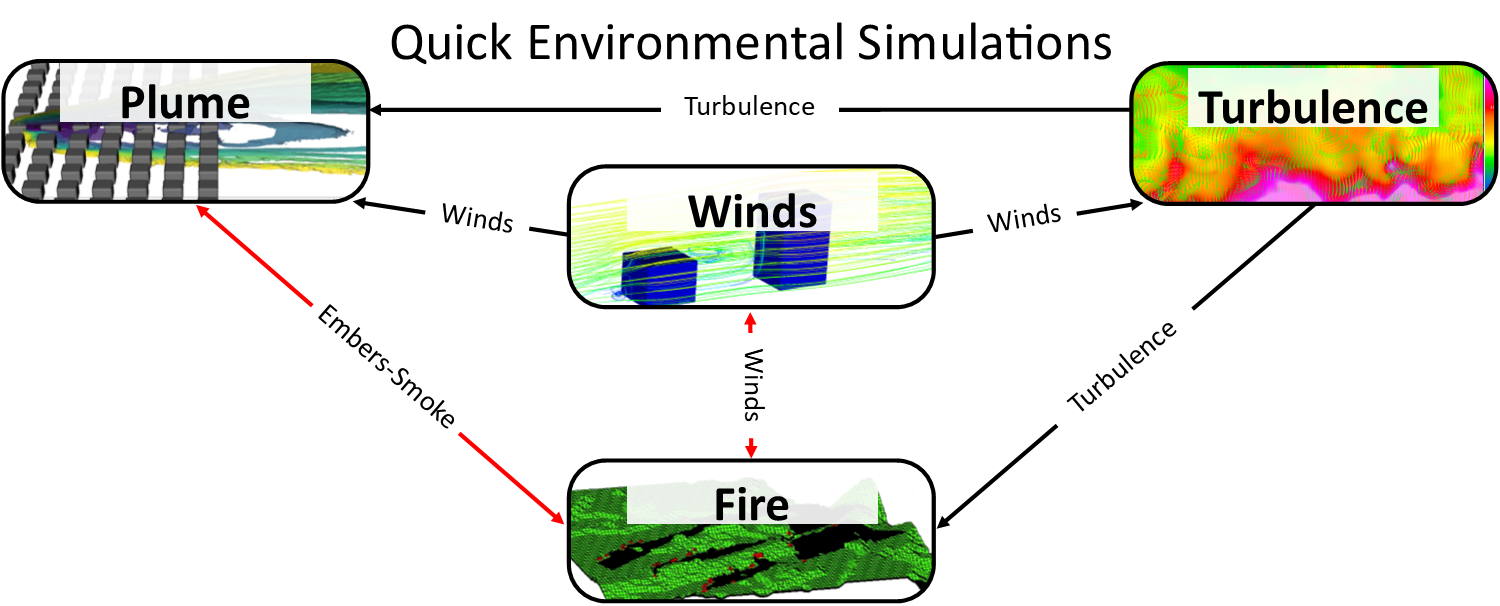
\includegraphics[width=16cm]{Images/QES_chart.png}
%\centering
%\caption{Schematic of the Quick Environmental System (QES) and the relationship between different elements of the system including data flow from one element to the other.}
%\label{fig:QES}
%\end{figure}

The fast-response three-dimensional diagnostic wind model written in C++, QES-Winds, is a rapid mass conserving wind-field solver. QES-Winds utilizes the concept of dynamic parallelism in CUDA to substantially accelerate wind simulations. Figure \ref{fig:Winds} shows a high-level flowchart for QES-Winds code.

\begin{figure}[H]
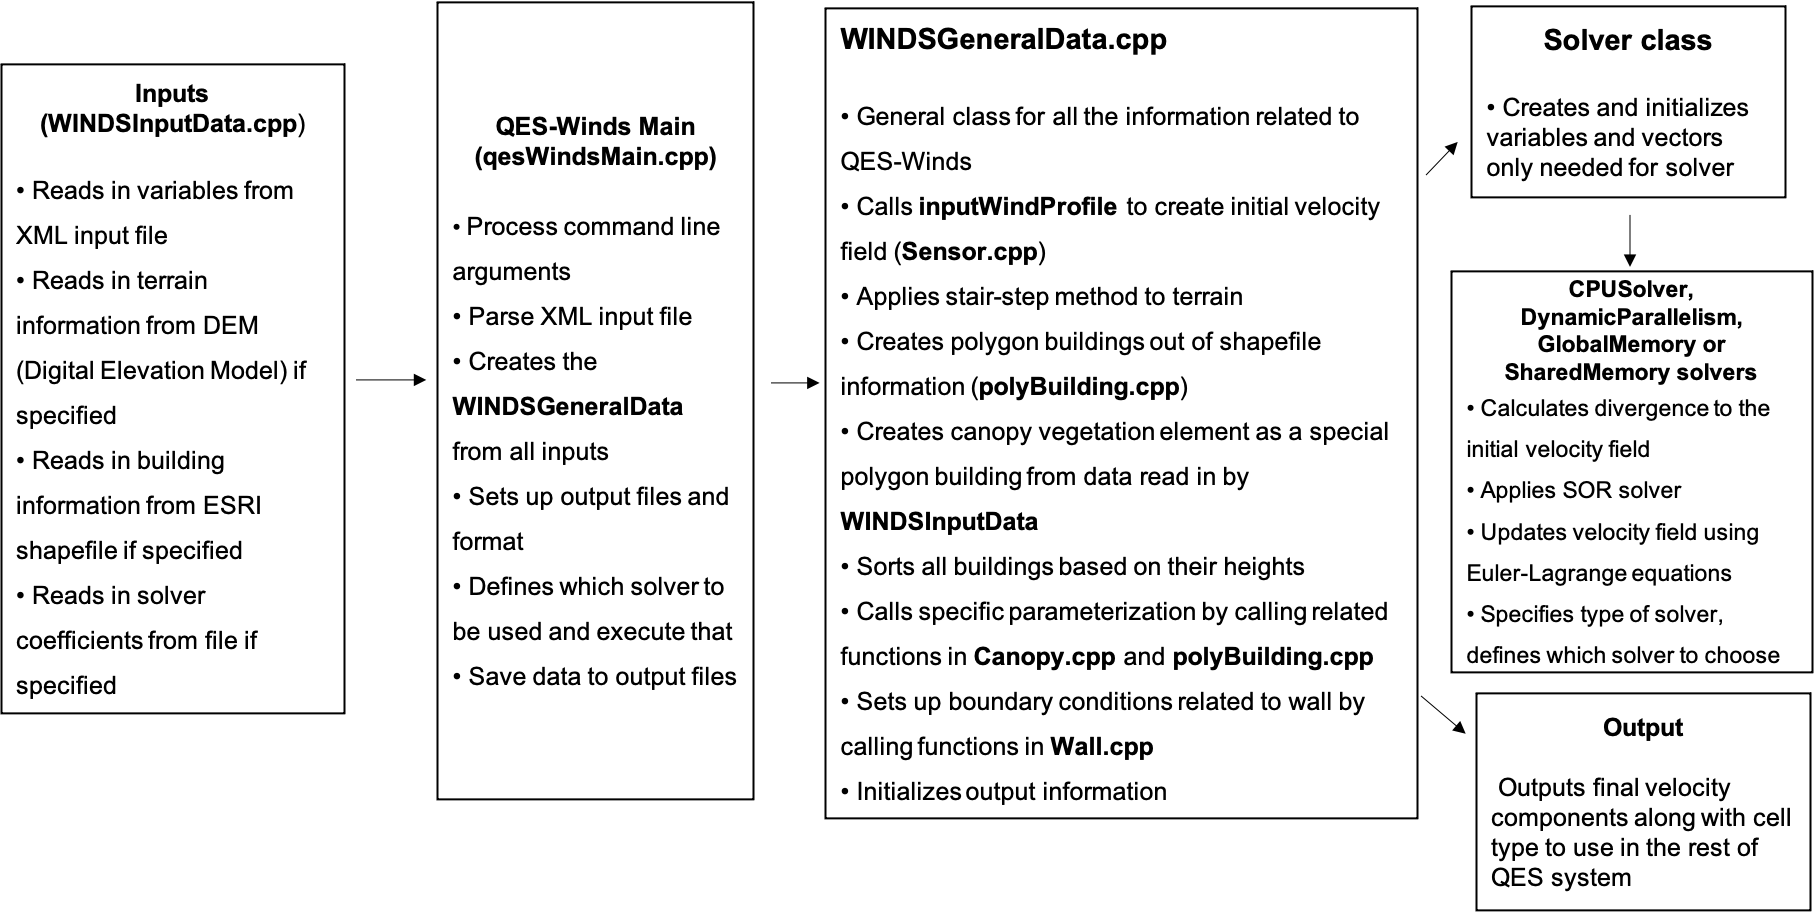
\includegraphics[width=17cm]{Images/QES_flowchart.png}
\caption{Flowchart for the QES-Winds wind solver}
\end{figure}

\section{QES-Winds Domain}

The first step in every computational code or package is to define the computational domain. The user can define the domain by specifying the number of cells in $x$, $y$ and $z$ directions as well as the cell size in each direction in the input file (XML file).

\subsection{XML Example}

The domain information (number of cells and cell size) are defined under the <simulationParameters> part of the XML file. Following is an example of a domain with $2$ km by $2$ km by $200$ m and resolution of $2$ m by $2$ m by $2$ m:

\begin{lstlisting}[language=XML]
<simulationParameters>
  	<domain> 1000 1000 100 </domain>					<!-- Number of cells in x,y and z directions-->
  	<cellSize> 2.0 2.0 2.0 </cellSize> 				<!-- Mesh resolution (meters)-->
</simulationParameters>
\end{lstlisting}

\section{Staggered Grid}

QES-Winds discretizes the computational domain using a staggered grid as shown in Figure \ref{fig:staggered_grid}. The velocity components ($u$, $v$ and $w$) are face-centered values and Lagrange multipliers ($\lambda$), divergence of the initial wind field ($R$) and solver coefficients ($e$, $f$, $g$, $h$, $m$ and $n$) are cell-centered variables. Because of nature of the finite difference method (depending on neighboring cells values), the first and last cells in $x$ and $y$ directions and the last cell in $z$ direction, are not updated in the solving process (their velocity remains as the same as the initial velocity field). For the same reason, there is a layer of ghost cells under the bottom surface to make velocity calculation in the first layer above the bottom surface possible. The values of the Lagrange multipliers for the ghost cells are set to the ones for the layer above the bottom surface to create a zero gradient for the Lagrange multipliers (boundary condition) as well as providing the neighboring cell for the finite difference method.

\begin{figure}[h!]
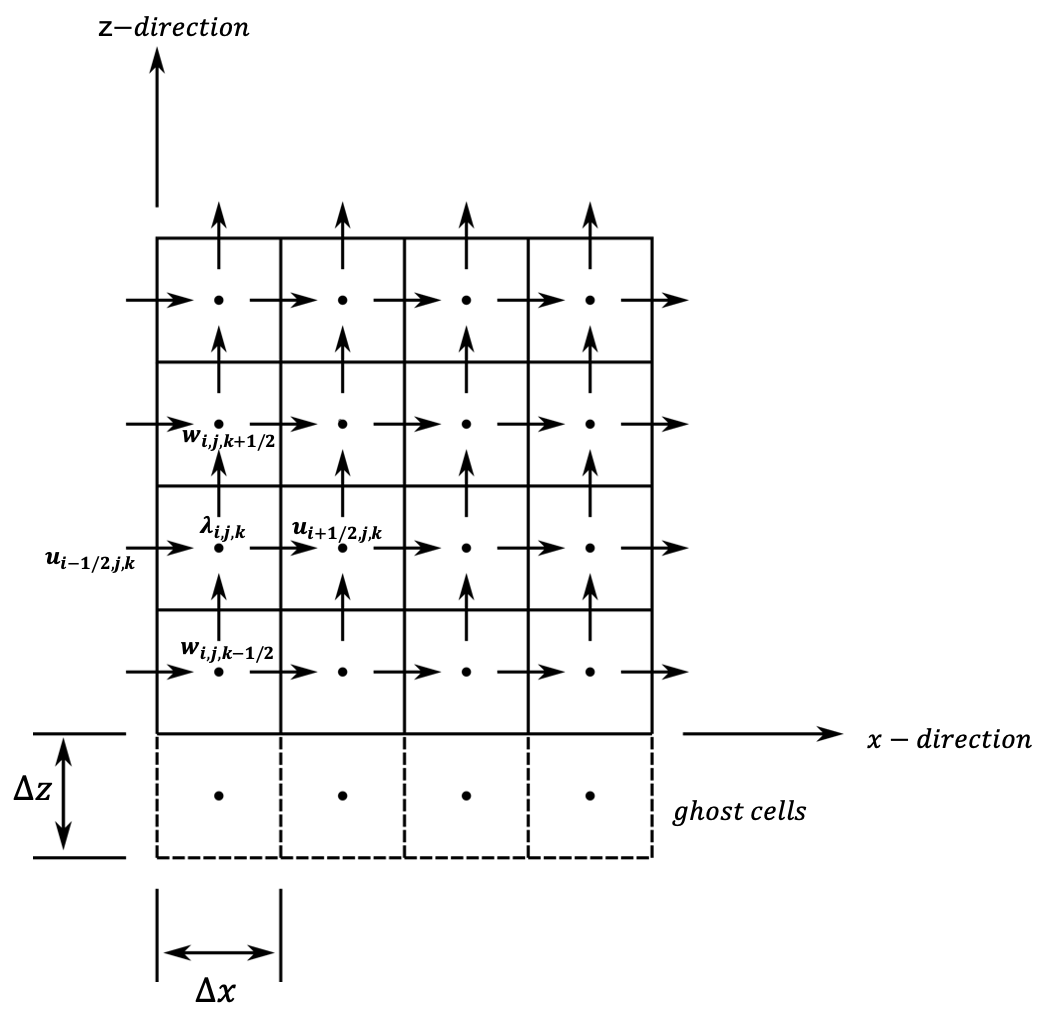
\includegraphics[width=11cm]{Images/staggered_grid_full.png}
\caption{Staggered grid representation of the domain and location of each variable.}
\end{figure}

\subsection{Halo Region}

If a solid element (building or terrain) overlaps with the QES domain boundaries, QES-Winds cannot model the wind field around the element correctly. In order to prevent this phenomenon, the user can add buffer zones to the sides of the domain when a terrain file or an ESRI shapefile is read into the code. Figure \ref{fig:halo} represents how the halo region is added to the domain around a Digital Elevation Model (DEM) or a shapefile.

\begin{figure}[h!]
\centering
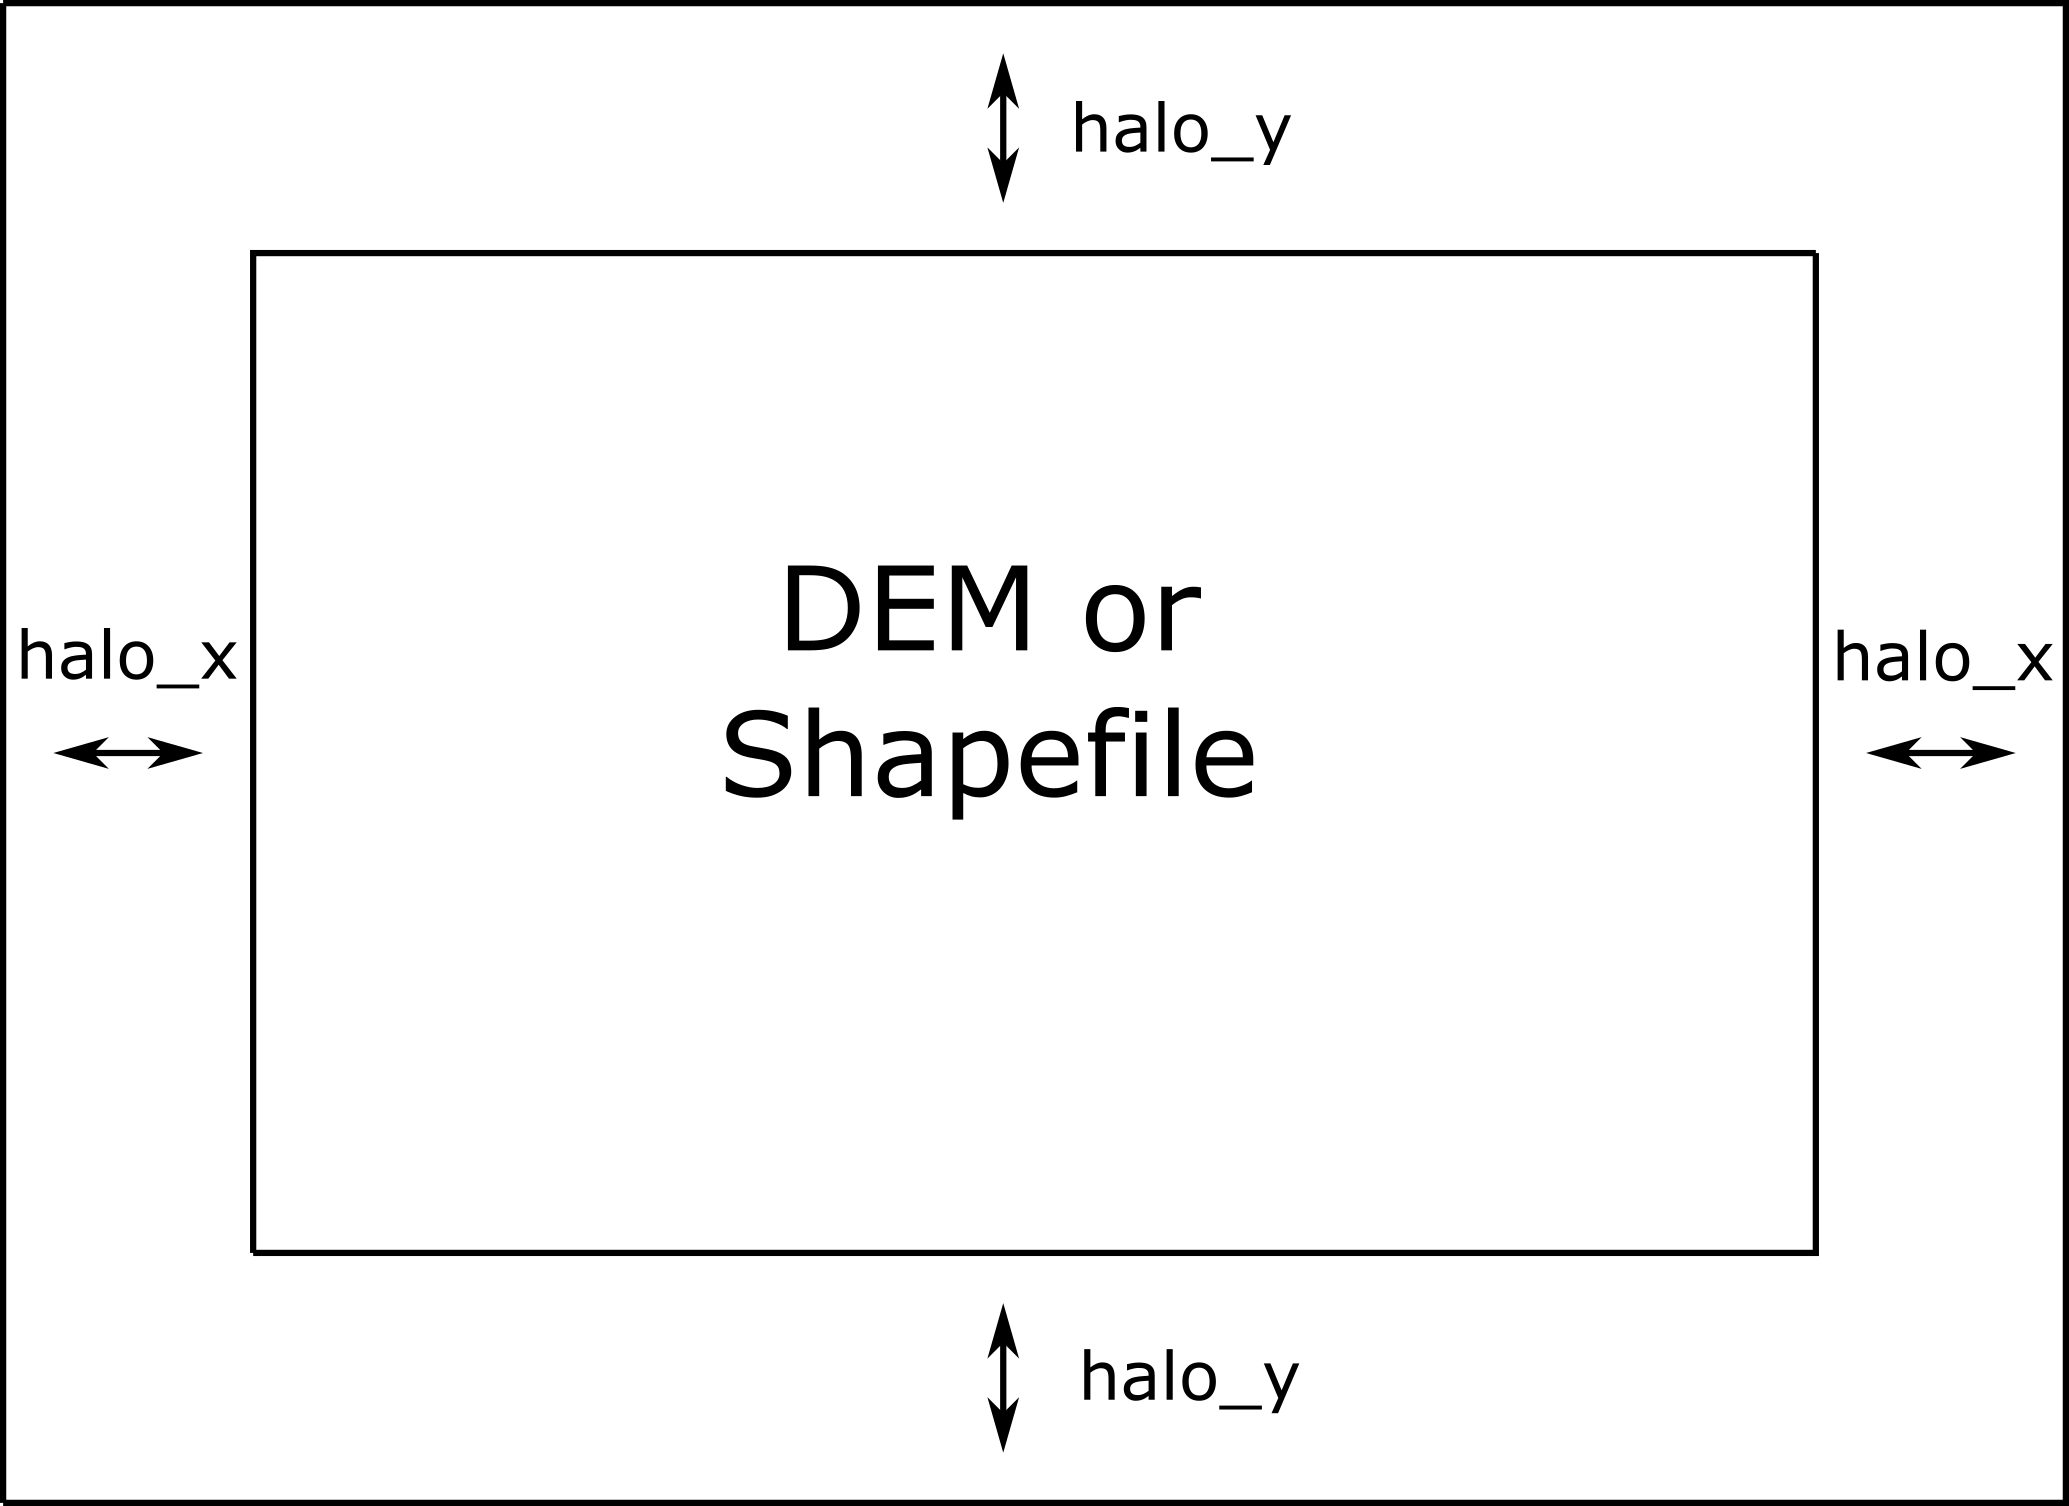
\includegraphics[width=11.0cm,keepaspectratio]{Images/domain_halo.png}
\caption{Representation of halo region around the domain.}
\end{figure}

In order to define length of the halo zone in $x$ and $y$ direction, the user can use <halo\textunderscore x> and <halo\textunderscore y> under <simulationParameters>. When the halo zone is defined, the length of the domain ($nx*dx$) and ($ny*dy$), should be greater than or equal to length of the DEM or shapefile in each direction plus twice the length of the halo in $x$ and $y$ directions, respectively.

\begin{lstlisting}[language=XML]
<simulationParameters>
  	<halo_x> 20.0 </halo_x>						<!-- Halo region added to x-direction of domain (at the beginning and the end of domain) (meters)-->
  	<halo_y> 30.0 </halo_y>						<!-- Halo region added to y-direction of domain (at the beginning and the end of domain) (meters)-->
</simulationParameters>
\end{lstlisting}

\section{Digital Elevation Model (DEM) and ESRI Shapefile}

The current version of QES-Winds has been written to allow commonly available terrain and building geometry datasets to be used for simulations. In this section, various input file formats for QES-Winds will be covered.

\subsection{Terrain Features}

Using the Geospatial Data Abstraction Library (GDAL; \href{https://www.gdal.org}{https://www.gdal.org}), we are able to load geo-referenced datasets of terrain so that the simulations can include the effects of hills, valleys, and mountains. In the current version of the code, we can load Digital Elevation Model (DEM) files for different physical locations.

Using the Digital Elevation Model (DEM) file loaders in our code base, we have loaded and tested multiple different terrain data sets. As a first test, we loaded a DEM of Askervein Hill. This is an isolated hill in Scotland where field experiments have been conducted and data for testing and evaluation exists (\cite{taylor1987askervein,mickle1988askervein}). The simulation with Askervein Hill was run without any complex terrain flow parameterizations. The Askervein Hill dataset is $6023.43$ m by $6023.43$ m. The hill height is approximately $124$ m tall. Figure \ref{fig:askervein} indicates the cell type contour for the Askervin hill test case in a vertical plane at $y = 3000$ m (part (a)), and a horizontal plane at $z=20$ m (part (b)). These plots show the ability of QES-Winds to read in and process DEM files. The cell type value $1$ (blue) represents the air cells while value $2$ (red) indicates the terrain cells.

\begin{figure}[H]
    \begin{subfigure}{\textwidth}
    \centering
    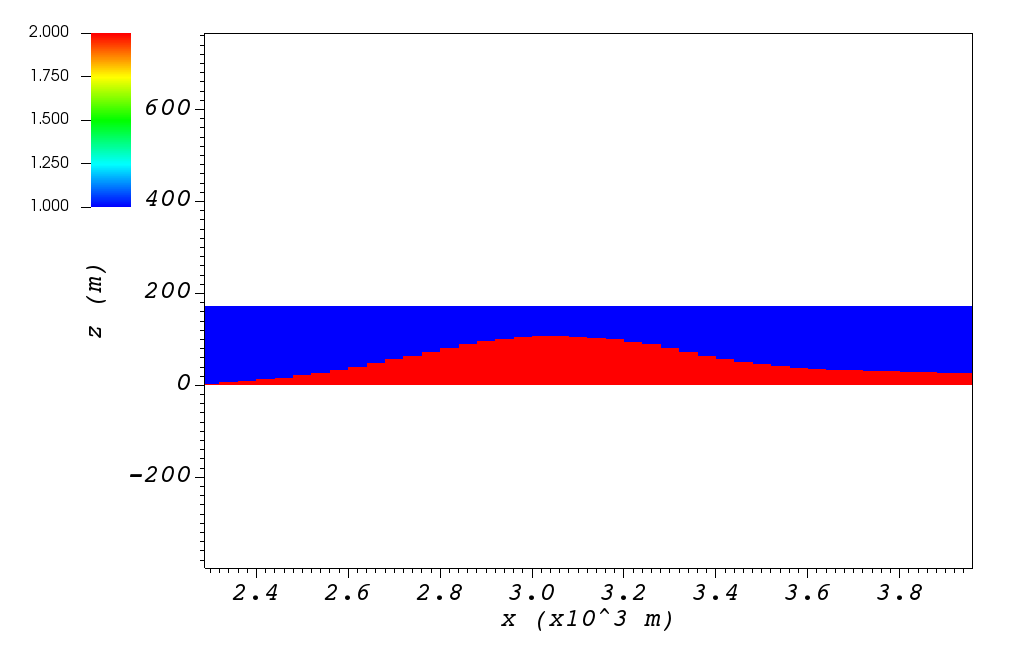
\includegraphics[width=13.0cm,keepaspectratio]{Images/askervein_y_3000_icell.png}
    \caption{}
    \end{subfigure}
    \begin{subfigure}{\textwidth}
    \centering
    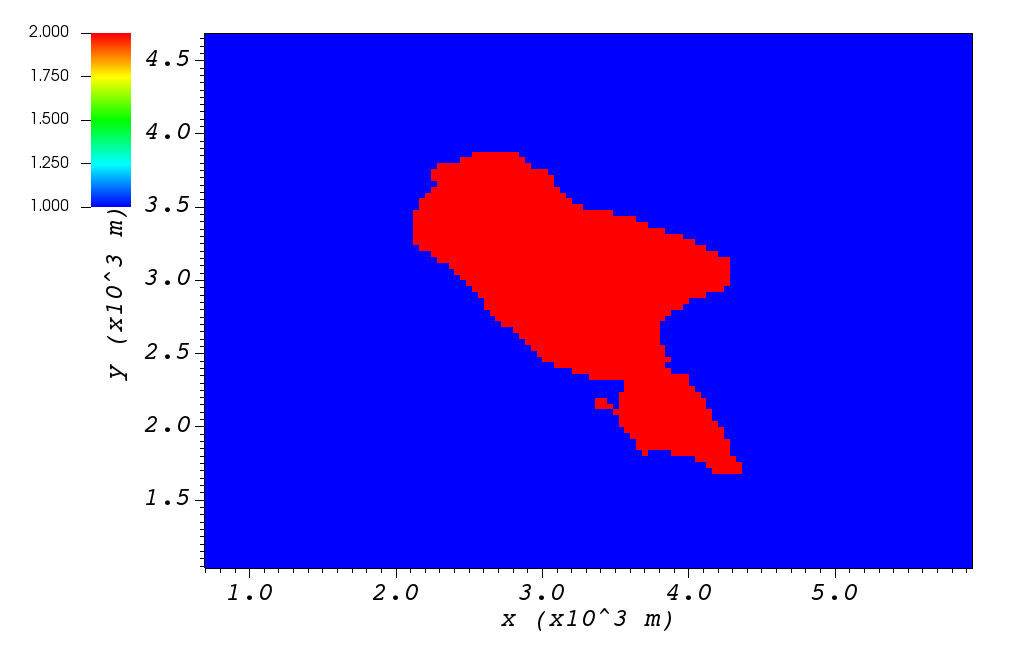
\includegraphics[width=13.0cm,keepaspectratio]{Images/askervein_z_20_icell.png}
    \caption{}
    \end{subfigure}
    \caption{Cell type contour for the Askervin hill test case in a (a) vertical plane at $y=3000$ m, (b) horizontal plane at $z=20$ m. The cell type value $1$ (blue) represents the air cells while value $2$ (red) indicates the terrain cells.}
\end{figure}

The user can define the address to the DEM using <DEM> variable under the <simulationParameters> part in the XML file:

\begin{lstlisting}[language=XML]
<simulationParameters>
  	<DEM>../scratch/DEM/askervein.tif</DEM>				<!-- Address to DEM location-->
</simulationParameters>
\end{lstlisting}

\subsubsection{Process Part of DEM}

In some cases, user wants to load a giant DEM but only process part of the file. This is possible in QES-Winds by defining the origin of QES domain inside the DEM borders and the size of the QES domain. Figure \ref{fig:DEM_cut} shows a schematic of how the QES domain can be defined inside a DEM file and only process that part.

\begin{figure}[h!]
\centering
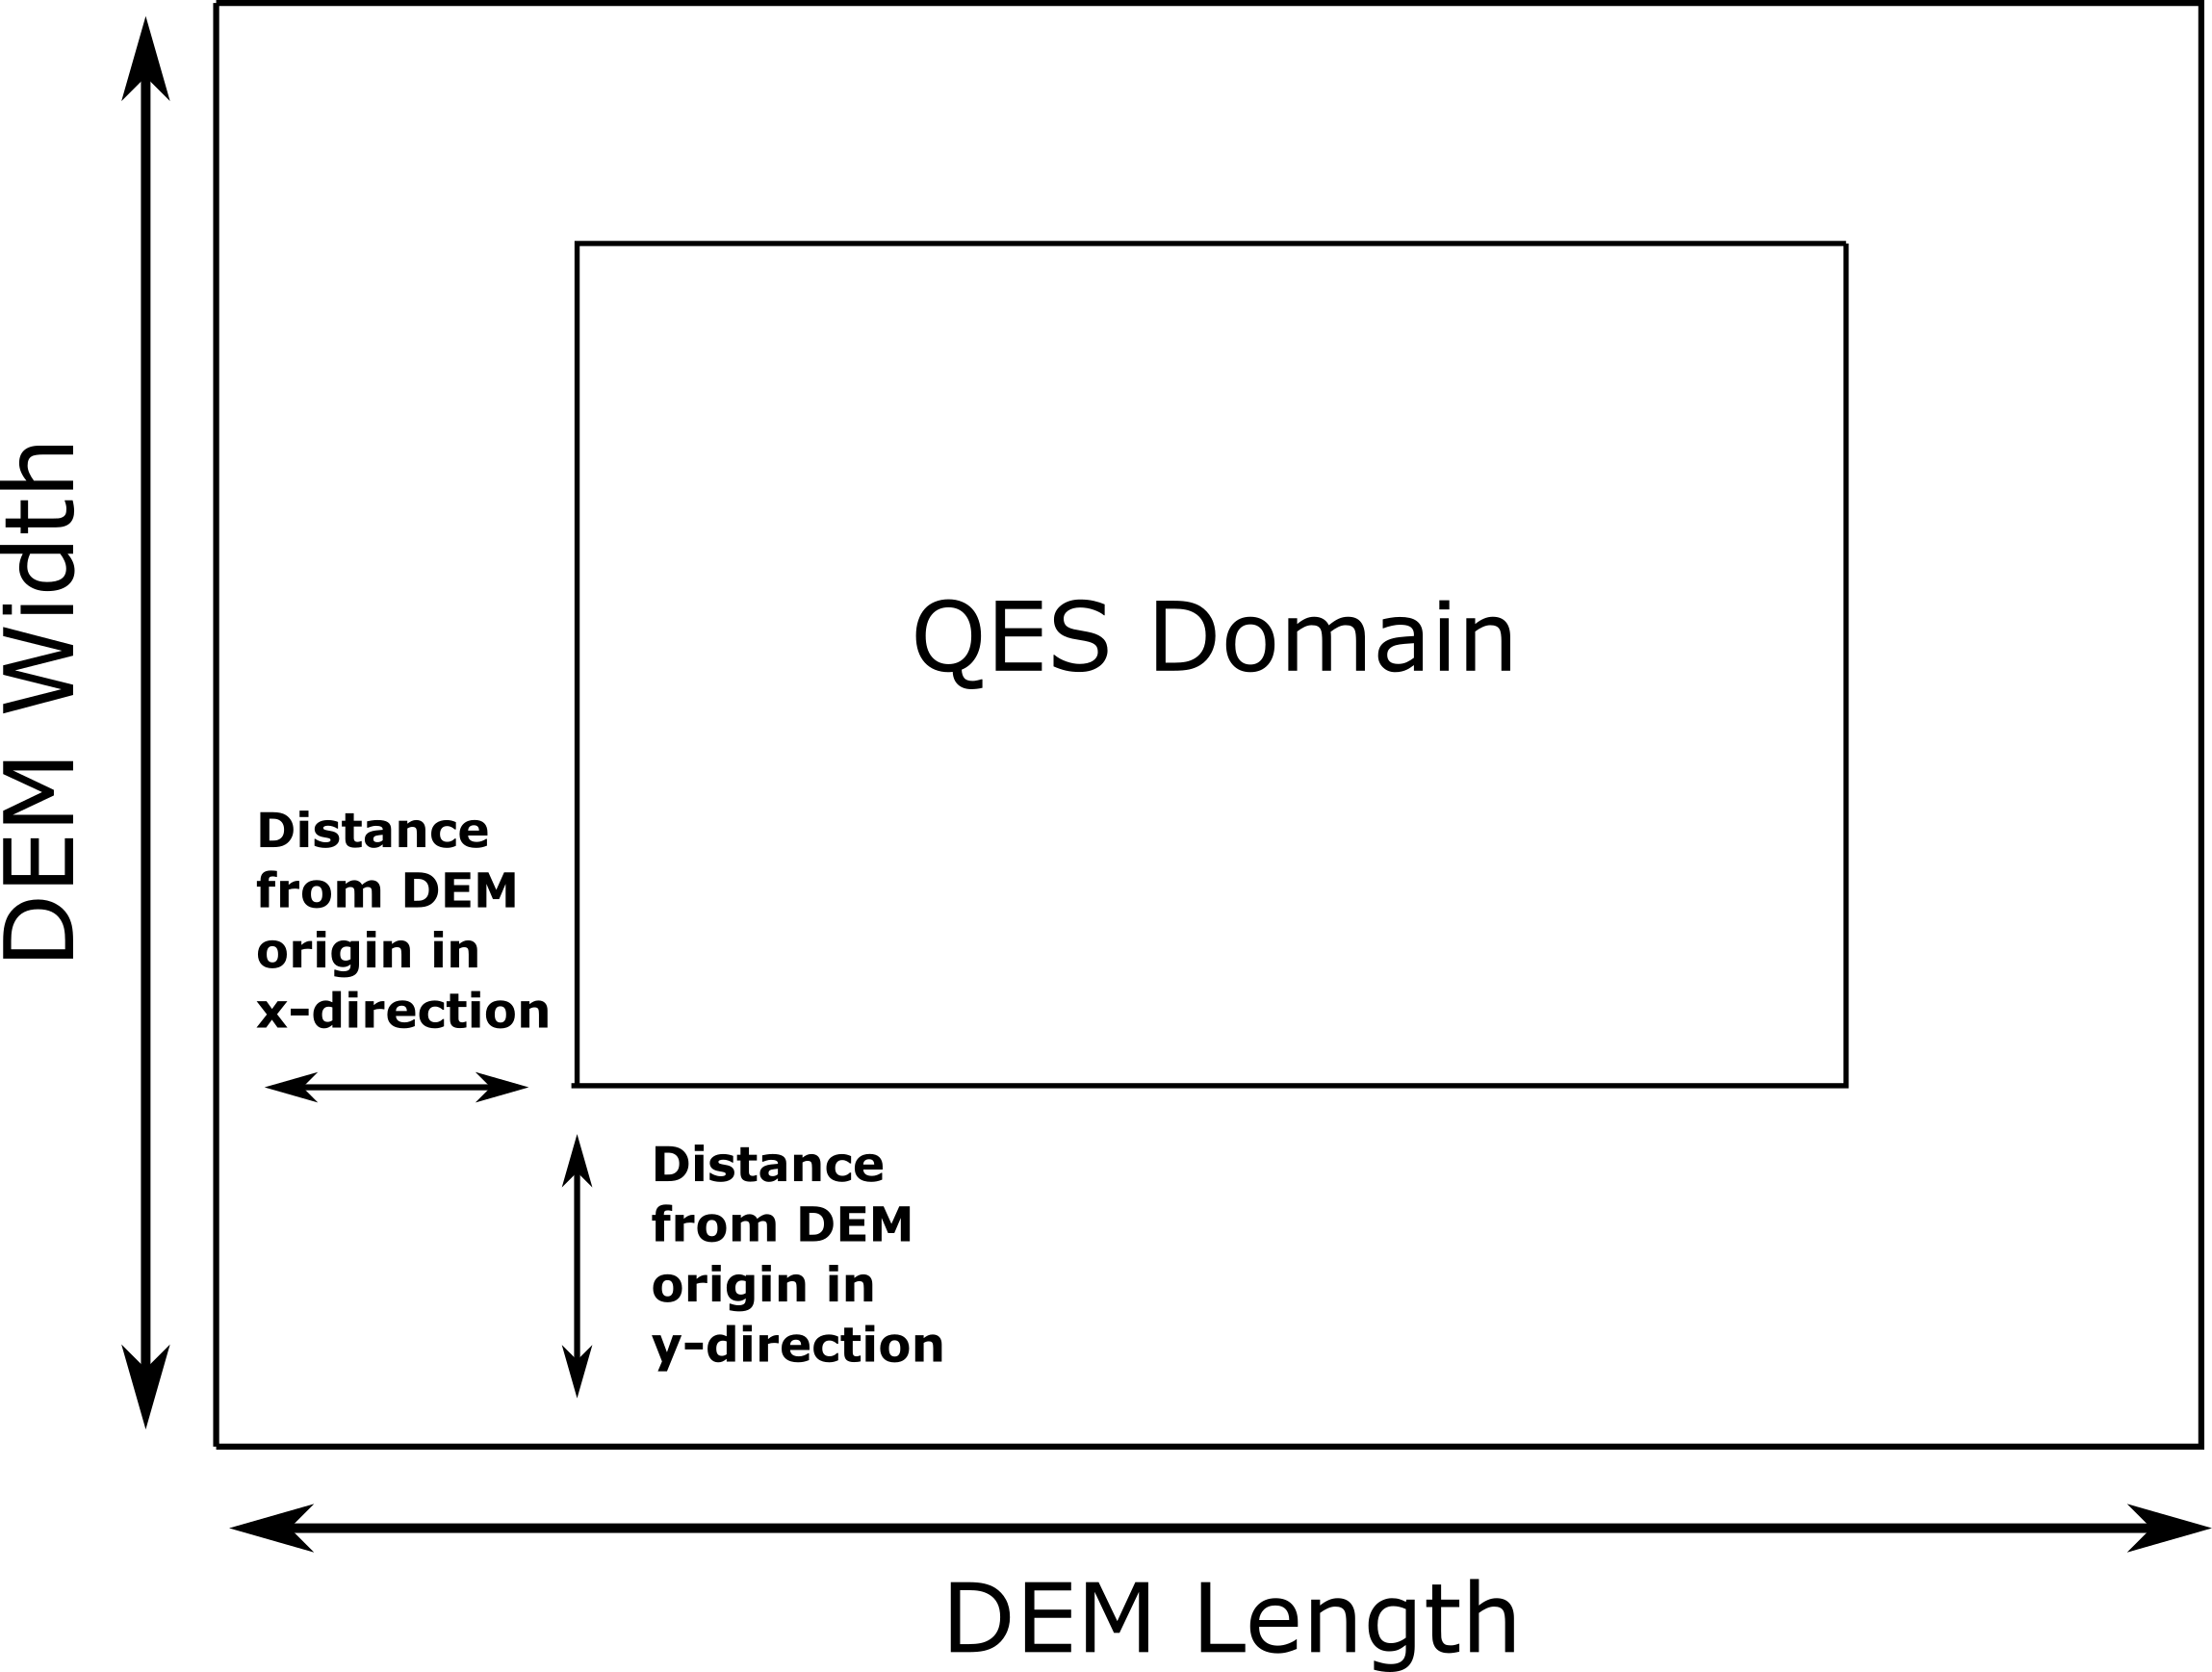
\includegraphics[width=13.0cm,keepaspectratio]{Images/DEM_cut.png}
\caption{Schematic of how the QES domain can be defined inside a DEM file and only process that part. }
\end{figure}

There are two options to determine the location of the origin of QES domain inside the DEM borders:

\begin{enumerate}
\item Specifying the distance of the QES origin with respect to bottom left corner of the DEM file. This can be done by setting the value of <originFlag> to $0$ and defining distances (in meters) in $x$ and $y$ directions using <DEMDistancex> and <DEMDistancey>, respectively.

\begin{lstlisting}[language=XML]
<simulationParameters>
  	<originFlag> 0 </originFlag>					<!-- Origin flag (0- DEM coordinates (default), 1- UTM coordinates) -->
	  <DEMDistancex> 1000.0 </DEMDistancex> 				<!-- x component (m) of origin in DEM coordinates (if originFlag = 0) -->
	  <DEMDistancey> 1000.0 </DEMDistancey> 				<!-- y component (m) of origin in DEM coordinates (if originFlag = 0) -->
</simulationParameters>
\end{lstlisting}

\item Defining the location of the QES domain origin in the Universal Transverse Mercator (UTM) coordinates by setting the value of <originFlag> to $1$ and determining <UTMx> and <UTMy> of the origin in $x$ and $y$ directions, respectively.

\begin{lstlisting}[language=XML]
<simulationParameters>
  	<originFlag> 1 </originFlag>					<!-- Origin flag (0- DEM coordinates (default), 1- UTM coordinates) -->
	  <UTMx> 595469.6122881 </UTMx> 					<!-- x component (m) of origin in UTM DEM coordinates (if originFlag = 1)-->
	  <UTMy> 6336281.9538635 </UTMy> 					<!-- y component (m) of origin in UTM DEM coordinates (if originFlag = 1)-->
</simulationParameters>
\end{lstlisting}

\end{enumerate}

\subsection{Automated City Building}

A new shapefile reader function has been added to QES-Winds, which provides the capacity to load the ESRI shapefiles using GDAL (Geospatial Data Abstraction Library) libraries. After the building footprints and heights are loaded from ESRI shapefiles, QES-Winds creates polygon buildings and applies appropriate parameterization to them. Figure \ref{fig:okc_qgis} shows an example ESRI shapefile can be read into QES-Winds, Central Business District (CBD) of Oklahoma City shapefile, subject to JU2003 experimental campaign \cite{allwine2006joint}, plotted using the freely available software QGIS (\href{https://qgis.org}{https://qgis.orgg}). The cell type contour for the Oklahoma City test case in a horizontal plane at $z=3$ m is shown in Figure \ref{fig:okc_icell}. This plot indicates the ability of QES-Winds to read in and process ESRI shapefiles. The cell type value $0$ (blue) represents the building cells while value $1$ (red) indicates the air cells.

\begin{figure}[H]
\centering
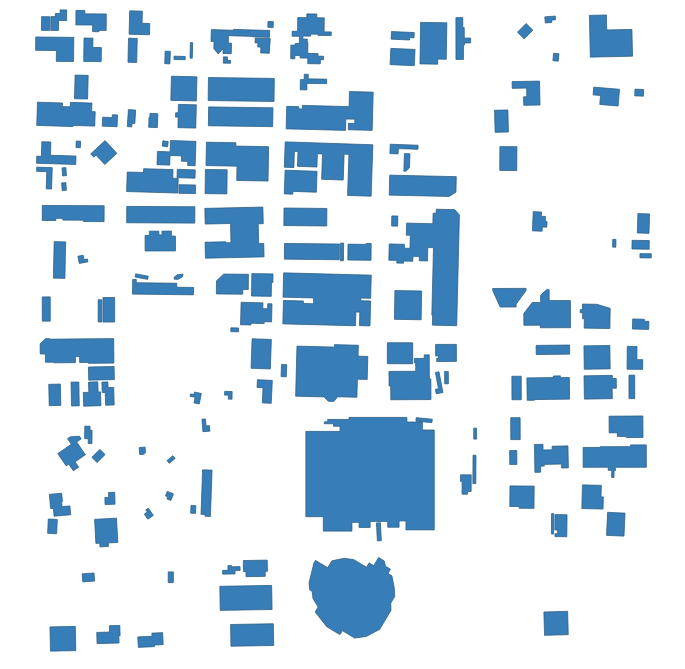
\includegraphics[width=13.0cm,keepaspectratio]{Images/OKC.png}
\caption{Central Business District (CBD) of Oklahoma City shapefile, subject to JU2003 experimental campaign \cite{allwine2006joint}, plotted using the freely available software QGIS.}
\end{figure}

\begin{figure}[H]
\centering
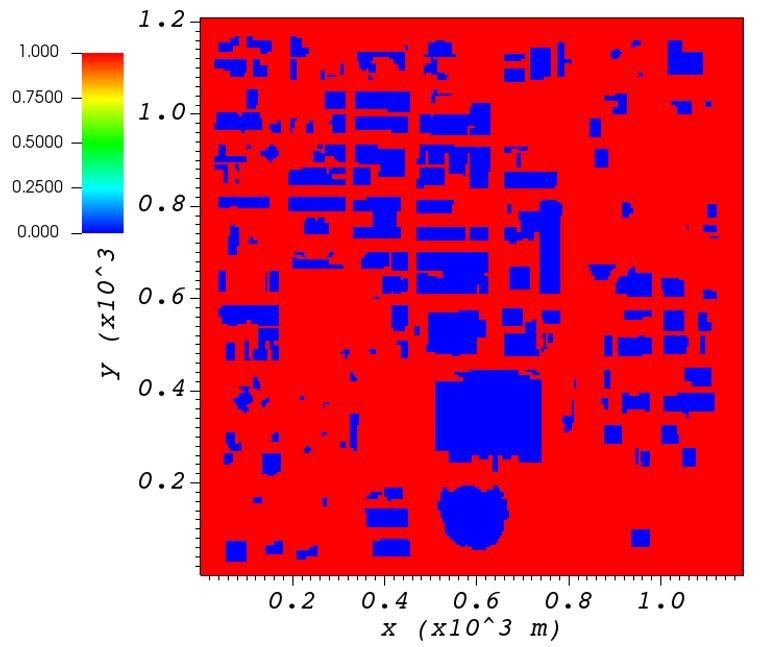
\includegraphics[width=\textwidth,keepaspectratio]{Images/oklahoma_z_3_icell.png}
\caption{Cell type contour for the Oklahoma City test case in a horizontal plane at $z=3$ m. The cell type value $0$ (blue) represents the building cells while value $1$ (red) indicates the air cells.}
\end{figure}

The user can define the address to the shapefile using <SHP> variable as well as the name of the shapefile using the <SHPBuildingLayer> and the correlation factor between the height field of the shapefile and the actual height of the buildings using the <heightFactor> under <simulationParameters> part in the XML file:

\begin{lstlisting}[language=XML]
<simulationParameters>
  	<SHP>../data/GISFiles/OKCSmallDomain/OKCSmallDomainJU2003.shp</SHP>	<!-- Address to shapefile location-->
  	<SHPBuildingLayer>OKCSmallDomainJU2003</SHPBuildingLayer>
  	<heightFactor> 1.0 </heightFactor>				<!-- Height factor multiplied by the building height read in from the shapefile (default = 1.0)-->
</simulationParameters>
\end{lstlisting}

\subsection{Import Building From XML}
\label{sec:building}

Instead of reading in a ESRI shapefile, the user can import building information manually through the XML file. This can be done by using the <buildings> section of the XML file. The only option available for now is the rectangular building. Information required for defining a rectangular building are height, base height, length, width, location of the closest corner to the origin of domain and building rotational angle. Following is an example of a rectangular building with $40$ m as height, $0$ m as base height, $20$ m as length and width, closest corner to the origin located at $90$ m in $x$ and $y$ directions, and $0^{\circ}$ as rotation angle with respect to the North-South line. Also, $0.1$ m is defined as the surface roughness for all the building walls.

\begin{lstlisting}[language=XML]
<buildings>
	<wallRoughness> 0.1 </wallRoughness>
	<rectangularBuilding>
		<height> 40.0 </height>
		<baseHeight> 0 </baseHeight>
		<xStart> 90.0 </xStart>
		<yStart> 90.0 </yStart>
		<length> 20.0 </length>
		<width> 20.0 </width>
		<buildingRotation> 0.0 </buildingRotation>
	</rectangularBuilding>
</buildings>
\end{lstlisting}

\section{Initial Wind Field}

QES-Winds can read a single or multiple sensors for a specific test case. In this context, sensor means the velocity magnitude and direction at a single point or a single velocity profile to initialize the wind field. If there is only the wind velocity and direction at a single point, the user should specify what type of velocity profile they want to build from the measurement. There are three options available for the type of profile:

\begin{enumerate}
\item a logarithmic profile \cite{favaloro2008toward}:
\begin{equation}
\label{eq:log_law}
u_{log}(z) = u_{ref}\cdot\frac{ln(z/z_0)}{ln(z_{ref}/z_0)}
\end{equation}

\item a power law profile \cite{favaloro2008toward}:
\begin{equation}
\label{eq:power_law}
u_{pow}(z) = u_{ref}\cdot(z/z_{ref})^{z_0}
\end{equation}

\item an urban canopy profile \cite{favaloro2008toward,pardyjak2008near}:
\begin{equation}
\label{eq:urban_canopy_low}
u_{uc}(z)=\begin{cases}
u(H)\cdot\exp(\alpha(\frac{z}{H}-1)) & \text{if} z\leq H\\
u(H)\cdot\exp(\alpha(\frac{z}{H}-1))& \text{if} z > H.
\end{cases}
\end{equation}

where $u_{ref}$ is the measured velocity at measured height $z_{ref}$, $z_0$ is the surface
roughness. The lower portion of the urban canopy profile calculated where $\alpha$ is a factor that depends on canopy
element density (attenuation coefficient) and $u(H)$ is the computed velocity at height $H$. The upper portion of the urban canopy is a different form of a logarithmic profile where $u_*$ is the friction velocity,
$\kappa$ is the von Karman constant at ~0.4 and $d$ is the zero plane displacement.

\end{enumerate}

If there is only one sensor available in the computational domain, the code will extend the profile for that sensor uniformly to the whole domain. On the occasion of multiple sensors, QES-Winds utilizes a two-dimensional Barnes interpolation scheme \cite{koch1983interactive,booth2012validation} to interpolate velocity components at each cell height of the domain based on the weighted distance from each sensor.

\subsection{XML Setup}
\label{sec:sensor_xml}

There are two options available for defining sensor information:

\begin{enumerate}

\item The user can put all the sensor information in a separate XML file and define the address to the location of the sensor file using the <sensorName> variable.

\begin{lstlisting}[language=XML]
<metParams>
	<z0_domain_flag> 0 </z0_domain_flag>           			<!-- Distribution of surface roughness for domain (0-uniform (default), 1-custom -->
	<sensorName>../data/InputFiles/sensor.xml</sensorName>	<!-- Name of the sensor file with information for the sensor included -->
</metParams>
\end{lstlisting}
\noindent

\item The user can define all information required for creating a sensor by using the <sensor> variable inside the <metParams> section of the XML file.

The first part of the sensor information is the location of the sensor in domain. There are three options for it: 1) define the location in local coordinates of the QES domain.

\begin{lstlisting}[language=XML]
<metParams>
	<sensor>
	    <site_coord_flag> 1 </site_coord_flag> 			<!-- Sensor site coordinate system (1=QES (default), 2=UTM, 3=Lat/Lon) -->
      <site_xcoord> 1.0  </site_xcoord> 				<!-- x component of site location in QES domain (m) (if site_coord_flag = 1) -->
      <site_ycoord> 1.0 </site_ycoord> 				<!-- y component of site location in QES domain (m) (if site_coord_flag = 1)-->
	</sensor>
</metParams>
\end{lstlisting}
\noindent

\item The user can define the location in the Universal Transverse Mercator (UTM) coordinates. In this case, user also needs to define the origin of computational domain in the UTM coordinates.

\begin{lstlisting}[language=XML]
<simulationParameters>
  <UTMx> 634173 </UTMx> 						<!-- x component (m) of origin in UTM -->
	<UTMy> 3925360 </UTMy> 						<!-- y component (m) of origin in UTM -->
	<UTMZone> 14 </UTMZone> 						<!-- UTM zone that domain located -->
</simulationParameters>
\end{lstlisting}

\begin{lstlisting}[language=XML]
<metParams>
	<sensor>
	    <site_coord_flag> 2 </site_coord_flag> 			<!-- Sensor site coordinate system (1=QES (default), 2=UTM, 3=Lat/Lon) -->
      <site_UTM_x> 634175 </site_UTM_x> 				<!-- x components of site coordinate in UTM (if site_coord_flag = 2) -->
      <site_UTM_y> 3925362 </site_UTM_y> 				<!-- y components of site coordinate in UTM (if site_coord_flag = 2)-->
      <site_UTM_zone> 14 </site_UTM_zone> 				<!-- UTM zone of the sensor site (if site_coord_flag = 2)-->
	</sensor>
</metParams>
\end{lstlisting}
\noindent
\item The user can define the location in Latitude and Longitude coordinates. In this case, user also needs to define the origin of computational domain in the UTM coordinates.

\begin{lstlisting}[language=XML]
<simulationParameters>
  <UTMx> 634173 </UTMx> 						<!-- x component (m) of origin in UTM -->
	<UTMy> 3925360 </UTMy> 						<!-- y component (m) of origin in UTM -->
	<UTMZone> 14 </UTMZone> 						<!-- UTM zone that domain located -->
</simulationParameters>
\end{lstlisting}

\begin{lstlisting}[language=XML]
<metParams>
	<sensor>
	    <site_coord_flag> 3 </site_coord_flag> 			<!-- Sensor site coordinate system (1=QES (default), 2=UTM, 3=Lat/Lon) -->
      <site_lat> 35.46270 </site_lat> 				<!-- x components of site coordinate in Latitude (if site_coord_flag = 3) -->
      <site_lat> -97.52130 </site_lat> 				<!-- y components of site coordinate in Longitude (if site_coord_flag = 3)-->
	</sensor>
</metParams>
\end{lstlisting}

\end{enumerate}

The second part of sensor definition is choosing type of profile for different time steps, if applicable. The <timeSeries> variable is designed to define type of sensor profile in the sensor section for several time steps. There are four options for the input profile in QES-Winds:

\begin{enumerate}
\item Logarithmic velocity profile, based on Eq. \ref{eq:log_law}:

\begin{lstlisting}[language=XML]
<metParams>
	<sensor>
	    <timeSeries>						<!-- Start of timestep informastion for a sensor -->
       		<boundaryLayerFlag> 1 </boundaryLayerFlag> 		<!-- Site boundary layer flag (1-log (default), 2-exp, 3-urban canopy, 4-data entry) -->
       		<siteZ0> 0.1 </siteZ0> 					<!-- Site z0 -->
       		<reciprocal> 0.0 </reciprocal> 				<!-- Reciprocal Monin-Obukhov Length (1/m) -->
       		<height> 20.0 </height> 				<!-- Height of the sensor -->
       		<speed> 5.0 </speed> 					<!-- Measured speed at the sensor height -->
       		<direction> 270.0 </direction> 				<!-- Wind direction of sensor -->
    	 </timeSeries>
	</sensor>
</metParams>
\end{lstlisting}

Figure \ref{fig:log_profile} shows velocity magnitude contour with overlaying velocity vectors of initial velocity field created by the aforementioned example of the logarithmic profile.

\begin{figure}[H]
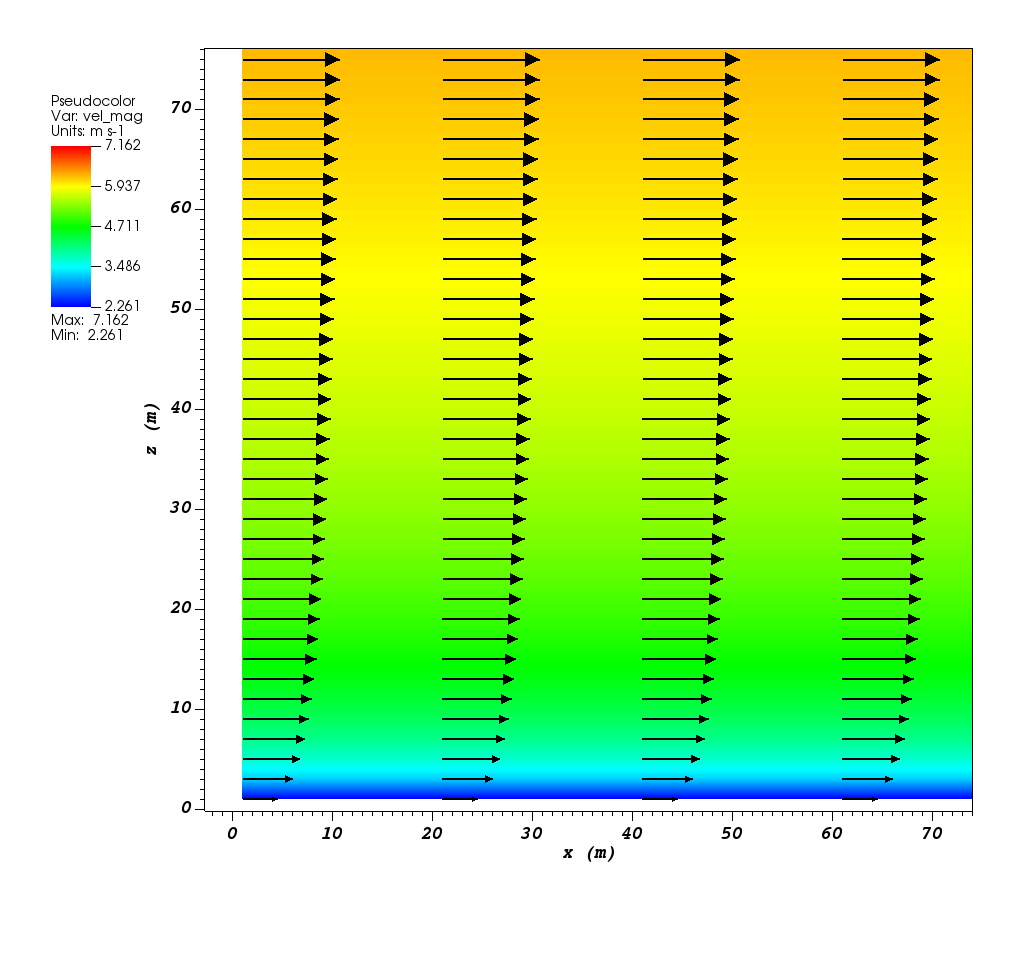
\includegraphics[width=\textwidth,keepaspectratio]{Images/log_y_101.png}
\caption{Velocity magnitude contour with overlaying velocity vectors in a vertical plane at $y=101$ m for initial velocity field created by the logarithmic profile.}
\end{figure}
\noindent

\item Exponential (power law) velocity profile, based on Eq. \ref{eq:power_law}:

\begin{lstlisting}[language=XML]
<metParams>
	<sensor>
	    <timeSeries>						<!-- Start of timestep informastion for a sensor -->
       		<boundaryLayerFlag> 2 </boundaryLayerFlag> 		<!-- Site boundary layer flag (1-log (default), 2-exp, 3-urban canopy, 4-data entry) -->
       		<siteZ0> 0.1 </siteZ0> 					<!-- Site z0 -->
       		<reciprocal> 0.0 </reciprocal> 				<!-- Reciprocal Monin-Obukhov Length (1/m) -->
       		<height> 20.0 </height> 				<!-- Height of the sensor -->
       		<speed> 5.0 </speed> 					<!-- Measured speed at the sensor height -->
       		<direction> 270.0 </direction> 				<!-- Wind direction of sensor -->
    	 </timeSeries>
	</sensor>
</metParams>
\end{lstlisting}

Figure \ref{fig:exp} shows velocity magnitude contour with overlaying  velocity vectors of the initial velocity field created by the aforementioned example of the exponential (power law) profile.

\begin{figure}[H]
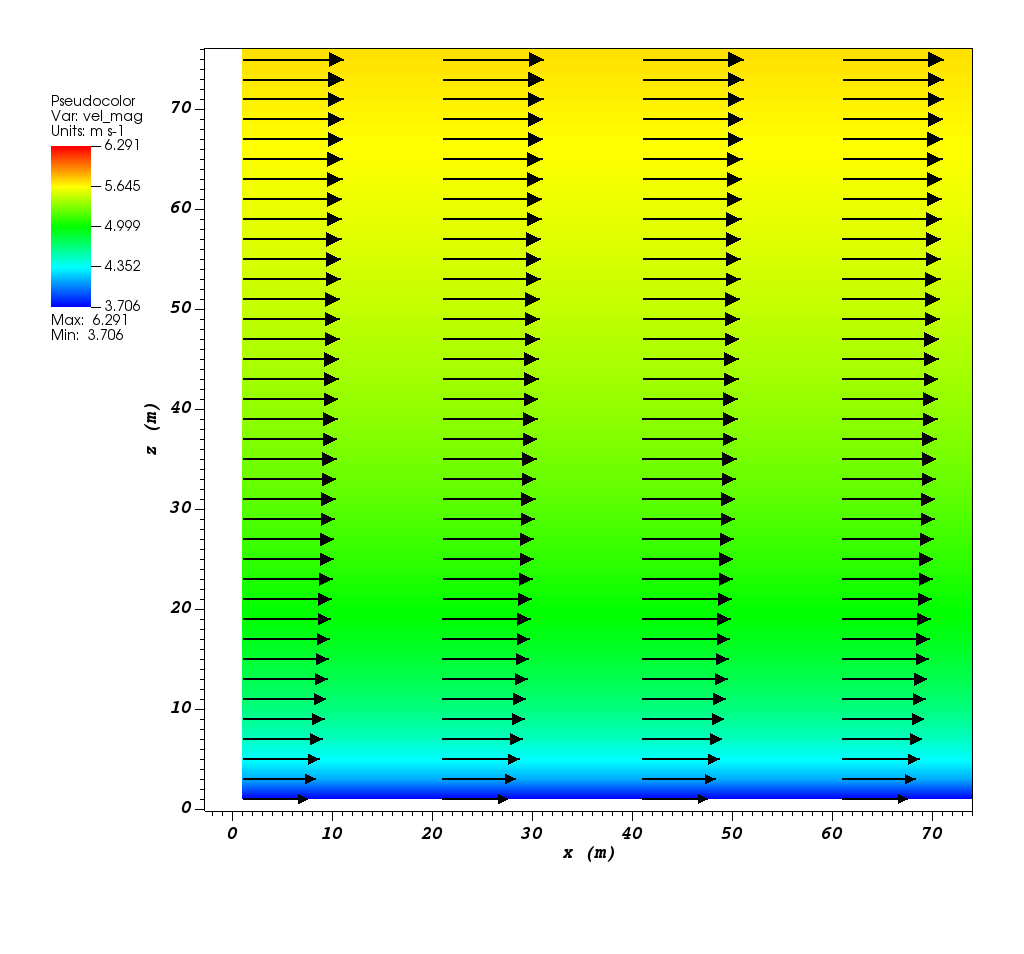
\includegraphics[width=\textwidth,keepaspectratio]{Images/exp_y_101.png}
\caption{Velocity magnitude contour with overlaying velocity vectors in a vertical plane at $y=101$ m for initial velocity field created by the exponential (power law) profile.}
\end{figure}
\noindent


\item Urban canopy velocity profile, based on Eq. \ref{eq:urban_canopy_low} and \ref{eq:urban_canopy_up}:

\begin{lstlisting}[language=XML]
<metParams>
	<sensor>
	    <timeSeries>						<!-- Start of timestep informastion for a sensor -->
       		<boundaryLayerFlag> 3 </boundaryLayerFlag> 		<!-- Site boundary layer flag (1-log (default), 2-exp, 3-urban canopy, 4-data entry) -->
       		<siteZ0> 0.1 </siteZ0> 					<!-- Site z0 -->
       		<reciprocal> 0.0 </reciprocal> 				<!-- Reciprocal Monin-Obukhov Length (1/m) -->
       		<height> 20.0 </height> 				<!-- Height of the sensor -->
       		<speed> 5.0 </speed> 					<!-- Measured speed at the sensor height -->
       		<direction> 270.0 </direction> 				<!-- Wind direction of sensor -->
		      <canopyHeight> 10.0 </canopyHeight>
		      <attenuationCoefficient> 1.0 </attenuationCoefficient>
    	 </timeSeries>
	</sensor>
</metParams>
\end{lstlisting}

Figure \ref{fig:canopy} shows velocity magnitude contour with overlaying  velocity vectors of the initial velocity field created by the aforementioned example of the urban canopy profile.

\begin{figure}[H]
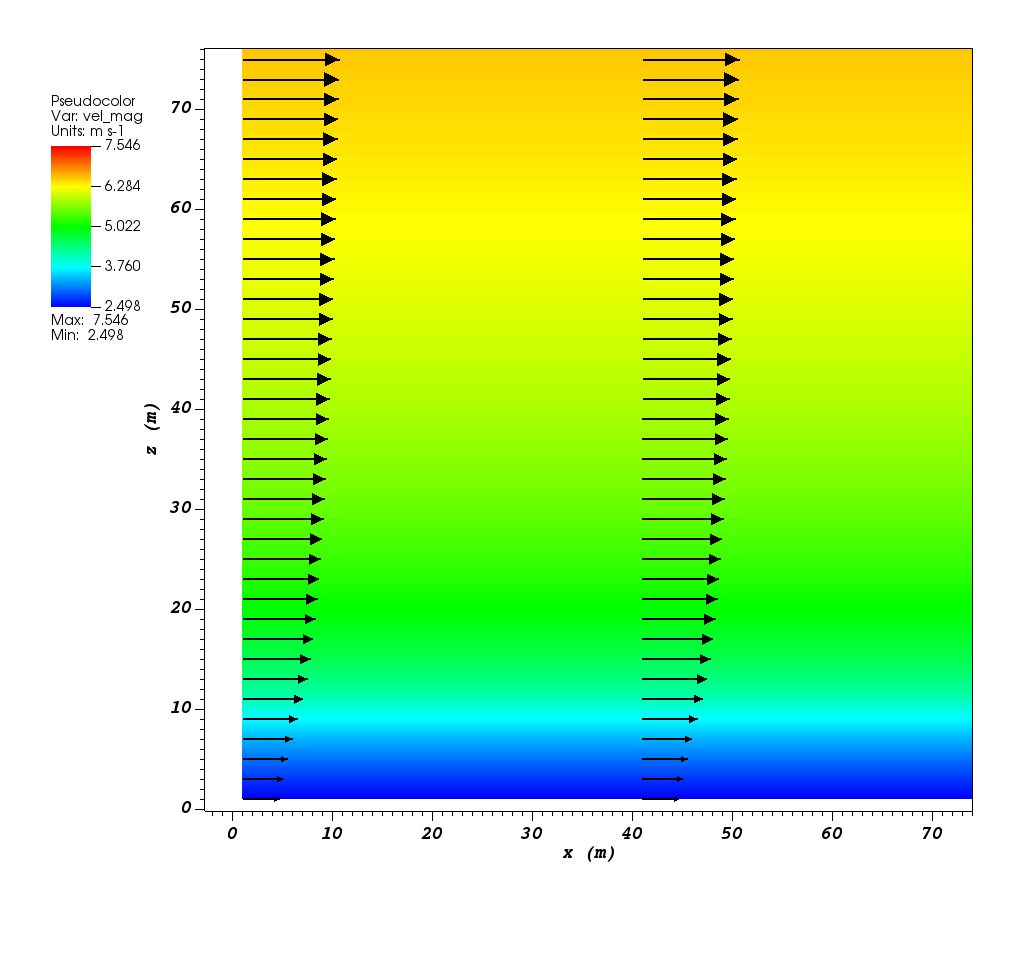
\includegraphics[width=\textwidth,keepaspectratio]{Images/canopy_y_101.png}
\caption{Velocity magnitude contour with overlaying velocity vectors in a vertical plane at $y=101$ m for initial velocity field created by the urban canopy profile.}
\end{figure}
\noindent

\item Data entry of the profile from an experimental tower with multiple sensors or from a numerical mesoscale weather prediction model like WRF \cite{powers2017weather}:

\begin{lstlisting}[language=XML]
<metParams>
	<sensor>
	    <timeSeries>						<!-- Start of timestep informastion for a sensor -->
       		<boundaryLayerFlag> 4 </boundaryLayerFlag> 			<!-- Site boundary layer flag (1-log, 2-exp, 3-urban canopy, 4-data entry) -->
          <siteZ0> 0.1 </siteZ0> 									<!-- Site z0 -->
          <reciprocal> 0.0 </reciprocal> 						<!-- Reciprocal Monin-Obukhov Length (1/m) -->
          <height> 30.7015 </height> 							<!-- Height of the sensor -->
          <height> 74.4169 </height>
          <height> 144.644 </height>
          <height> 197.455 </height>
          <height> 268.468 </height>
          <speed> 2.56922 </speed> 							<!-- Measured speed at the sensor height -->
          <speed> 2.55532 </speed>
          <speed> 2.33319 </speed>
          <speed> 2.16058 </speed>
          <speed> 1.98843 </speed>
          <direction> 323.283 </direction> 					<!-- Wind direction of sensor -->
          <direction> 327.377 </direction>
          <direction> 332.676 </direction>
          <direction> 337.649 </direction>
          <direction> 344.273 </direction>
    	</timeSeries>
	</sensor>
</metParams>
\end{lstlisting}

\end{enumerate}

\section{Empirical Parameterizations}

QES-Winds only conserves mass and no momentum equation is solved. As a result, the solution is a potential-flow solution (no shear effects). In order to add shear effects to our solution, empirical parameterizations are needed. These parameterizations are designed using results of experiments and computational simulations (e.g. \cite{singh2008evaluation,brown2013quic}). Buildings are the most important elements in urban areas. There are several parameterizations developed for different areas around the building. This section covers available parameterizations in QES-Winds along with their effects on the wind field.

test: \autoref{upwind-cavity} \autoref{leeside-cavity-and-far-wake}

\begin{lstlisting}[language=XML]
<buildingsParams>
    <wallRoughness>0.01</wallRoughness>  
    <!-- Rooftop flag (0-none, 1-log profile (default), 2-vortex) -->
    <rooftopFlag> 2 </rooftopFlag> 
    <!-- Upwind cavity flag (0-none, 1-Rockle, 2-MVP (default), 3-HMVP) -->
    <upwindCavityFlag> 2 </upwindCavityFlag> 	
    <!-- Street canyon flag (0-none, 1-Roeckle w/ Fackrel (default)) -->		
    <streetCanyonFlag> 1 </streetCanyonFlag> 	
    <!--Street intersection flag (0-off, 1-on) -->		
    <streetIntersectionFlag> 0 </streetIntersectionFlag> 
    <!-- Wake flag (0-none, 1-Rockle, 2-Modified Rockle (default), 3-Area Scaled) -->		
    <wakeFlag> 2 </wakeFlag> 					
	<!-- High-rise flag (0-off (default), 1-on) -->
    <highRiseFlag> 0 </highRiseFlag> 
    <!-- Sidewall flag (0-off, 1-on (default)) -->           
    <sidewallFlag> 0 </sidewallFlag> 				
    
    <!-- Address to shapefile location-->
    <SHPFile>SaltLakeCity/slc_cut.shp</SHPFile>	 
    <!-- Name of building layer in shapefile-->                       
    <SHPBuildingLayer>slc_cut</SHPBuildingLayer>     
    <!-- Name of building height field in shapefile -->                     
    <SHPHeightField>MEANHEIGHT</SHPHeightField>      
    <!-- Height factor multiplied by the building height in the shapefile (default = 1.0)-->                    
    <heightFactor> 1.0 </heightFactor>				        
  </buildingsParams>
\end{lstlisting}

\subsection{Upwind Cavity}\label{upwind-cavity}

Upwind cavity as described in \cite{nelson20085,bagal2004improved,gowardhan2010evaluation} is the parameterization representing upwind and stagnation effects of the building on the fluid flow. There are three options available for this type of parameterization in QES-Winds. The first option based on the parameterization proposed by R\"{o}ckle \cite{rockle1990bestimmung} and later Kaplan and Dinar \cite{kaplan1996lagrangian}. They defined an ellipsoid to represent what they call is the displacement zone in front of the building. The length of the displacement zone, $L_F$, is defined by: 
\begin{equation}
\frac{L_{\mathrm{F}}}{H}=\frac{2(W / H)}{1+0.8 W / H}
\label{eq:lf}
\end{equation}

The shape of the ellipsoid is estimated by:
\begin{equation}
\frac{X^{2}}{L_{\mathrm{F}}^{2}\left(1-(Z / 0.6 H)^{2}\right)}+\frac{Y^{2}}{W^{2}}=1
\label{eq:upwind}
\end{equation}
where $L$, $H$ and $W$ are length, width and height of the building, receptively.Finally, the initial velocity components in the displacement zone are set to zero.


Part (a) of Figure \ref{fig:upwind_1_vert} and Figure \ref{fig:upwind_1_horiz} show cell type contour to represent the area of effect of the R\"{o}ckle upwind cavity parameterization in a vertical plane at $y=100$ m and a horizontal plane at $z=5$ m, respectively. The upwind parameterizations is applied to a rectangular building defined in Section \ref{sec:building}. The initial guess field is constructed using a single sensor with logarithmic profile as defined in \ref{sec:sensor_xml}. Parts (b) and (c) of Figure \ref{fig:upwind_1_vert} and Figure \ref{fig:upwind_1_horiz} indicate velocity magnitude contour with overlaying velocity vectors of initial (part (b)) and final (part(c)) velocity fields in a vertical plane at $y=100$ m and a horizontal plane at $z=5$ m, respectively.

\begin{figure}[H]
    \centering
    \begin{subfigure}{\textwidth}
    \centering
    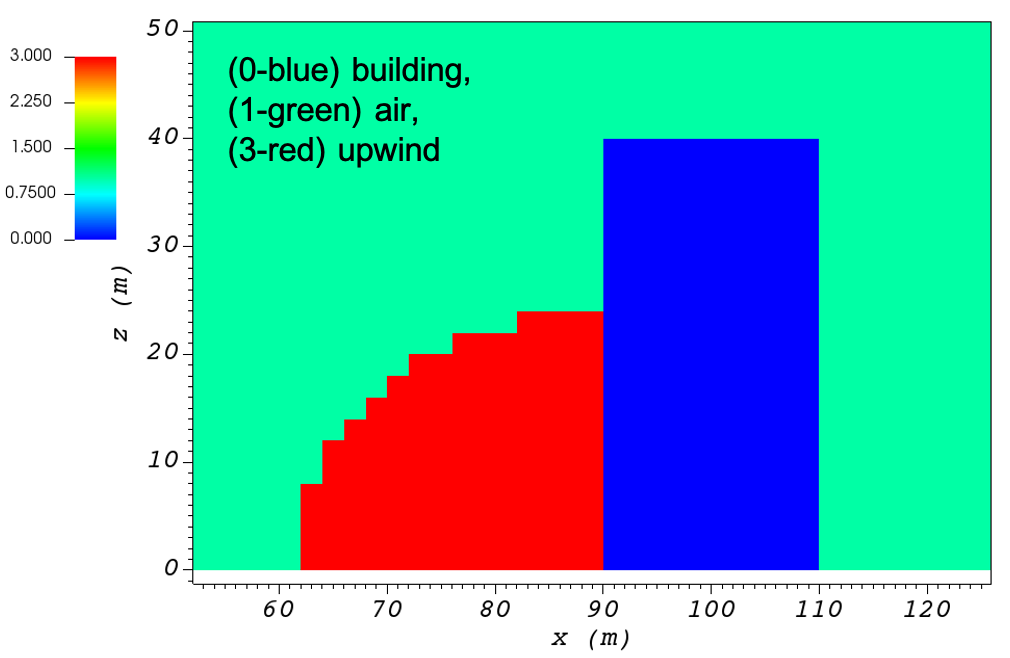
\includegraphics[width=10.3cm,keepaspectratio]{Images/upwind_y_100_1_init_icell.png}
    \caption{}
    \end{subfigure}
    \begin{subfigure}{\textwidth}
    \centering
    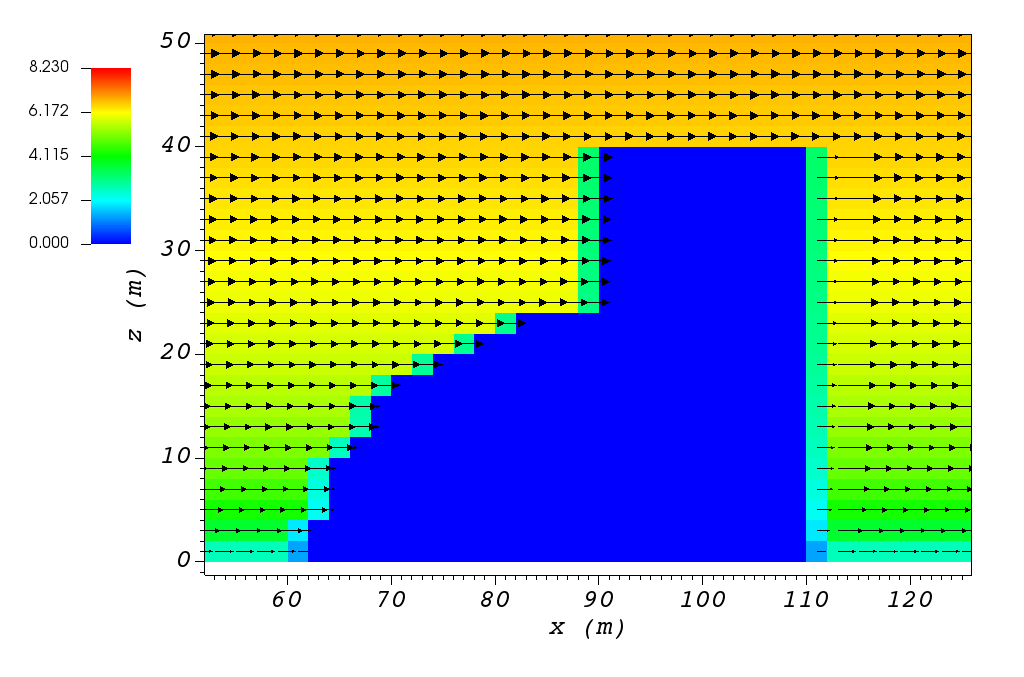
\includegraphics[width=11.0cm,keepaspectratio]{Images/upwind_y_100_1_init_vel.png}
    \caption{}
    \end{subfigure}
    \begin{subfigure}{\textwidth}
    \centering
    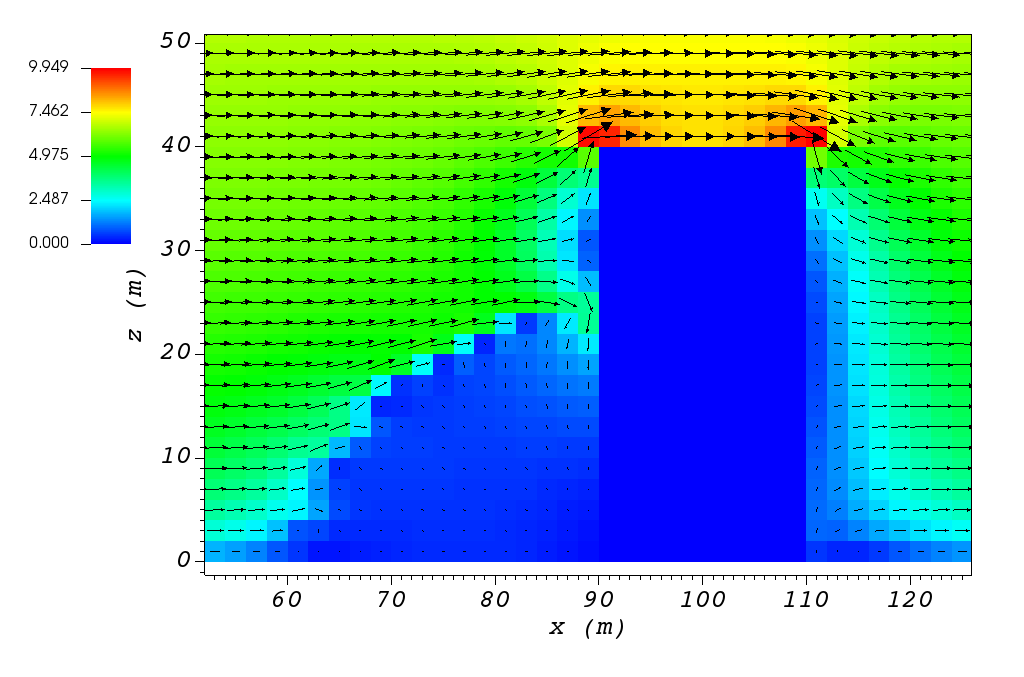
\includegraphics[width=11.0cm,keepaspectratio]{Images/upwind_y_100_1_final.png}
    \caption{}
    \end{subfigure}
    \caption{(a) Cell type contour to show the area of effect of the R\"{o}ckle upwind cavity parameterization in a vertical plane at $y=100$ m. Velocity magnitude contour with overlaying velocity vectors of (b) initial velocity field and (c) final velocity field, in a vertical plane at $y=100$ m.}
\end{figure}

\begin{figure}[H]
    \centering
    \begin{subfigure}{\textwidth}
    \centering
    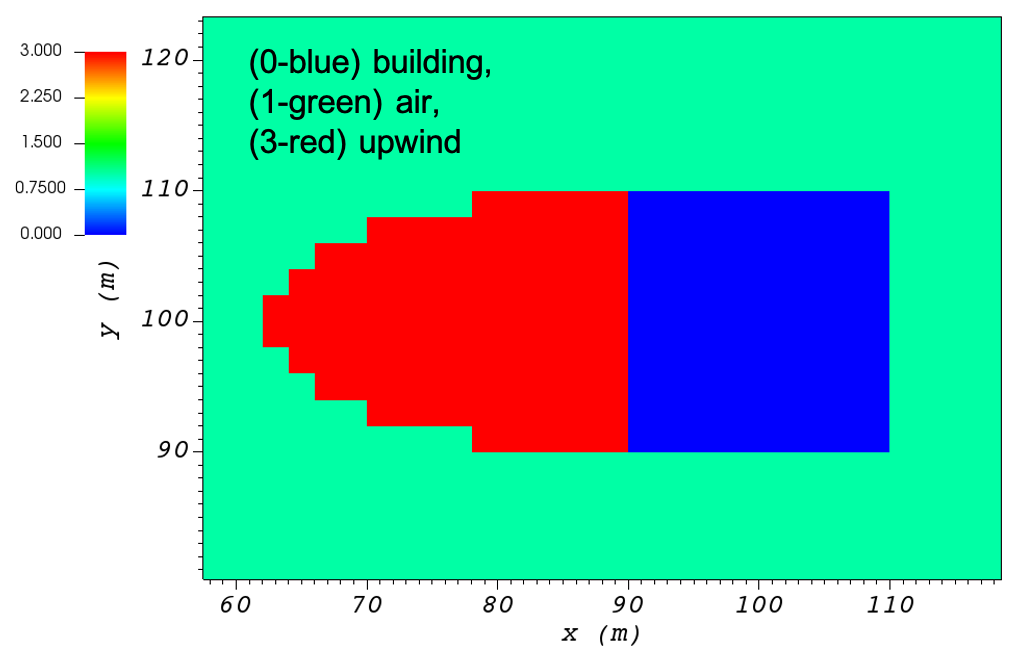
\includegraphics[width=10.3cm,keepaspectratio]{Images/upwind_z_5_1_init_icell.png}
    \caption{}
    \end{subfigure}
    \begin{subfigure}{\textwidth}
    \centering
    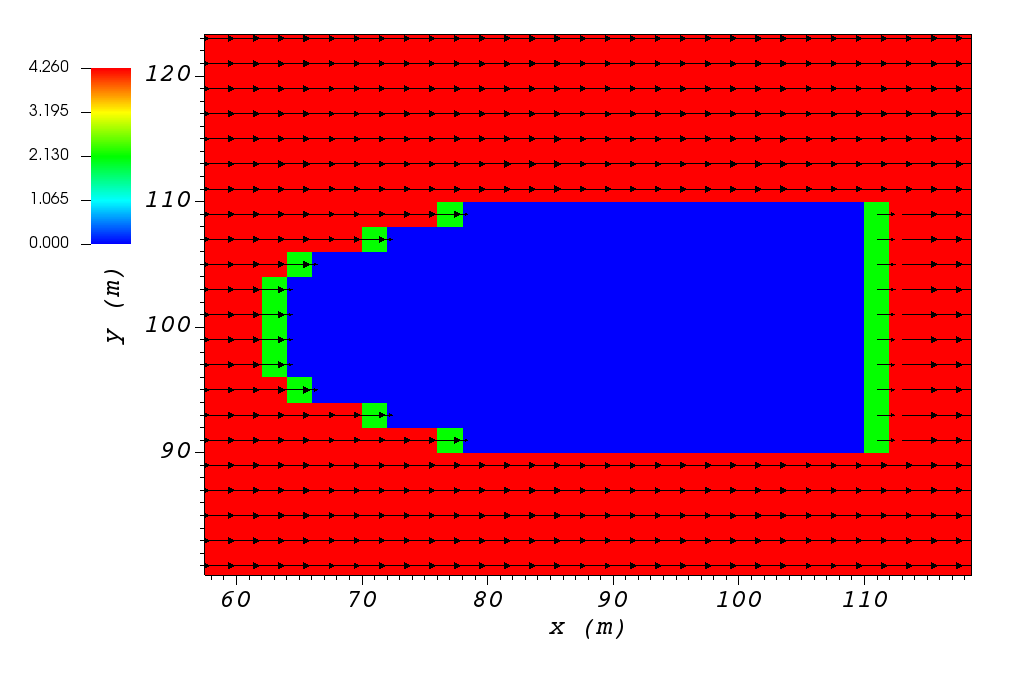
\includegraphics[width=11.0cm,keepaspectratio]{Images/upwind_z_5_1_init_vel.png}
    \caption{}
    \end{subfigure}
    \begin{subfigure}{\textwidth}
    \centering
    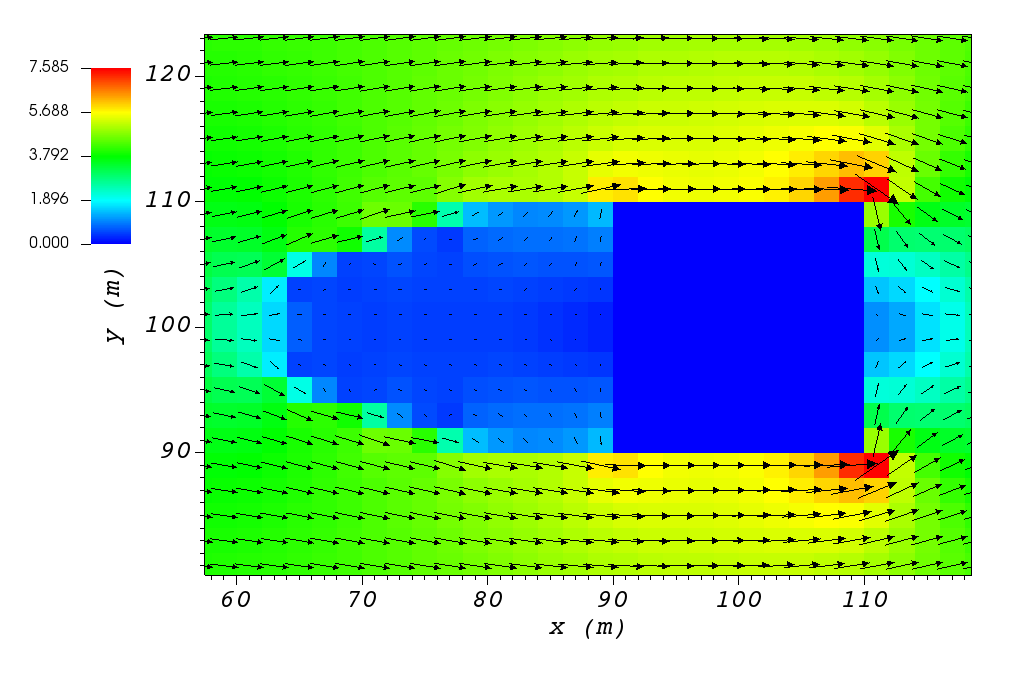
\includegraphics[width=11.0cm,keepaspectratio]{Images/upwind_z_5_1_final.png}
    \caption{}
    \end{subfigure}
    \caption{(a) Cell type contour to show the area of effect of the R\"{o}ckle upwind cavity parameterization in a horizontal plane at $z=5$ m. Velocity magnitude contour with overlaying velocity vectors of (b) initial velocity field and (c) final velocity field, in a horizontal plane at $z=5$ m.}
\end{figure}

The second option is called the Modified
Vortex Parameterization (MVP) and created by Bagal et al. \cite{bagal2004improved}. In this parameterization, the length of the displacement zone, $L_F$, is calculated by Eq. \ref{eq:lf_MVP}. The MVP parameterization defines two ellipsoids instead of one: In the outer ellipsoid,  velocities are reduced to $40\%$ of their initial values while in the inner region, velocity components are set to zero \cite{nelson20085}. Both ellipsoids are extended to $0.6$ of the building height.

\begin{equation}
\frac{L_{\mathrm{F}}}{H}=\frac{1.5(W / H)}{1+0.8 W / H}
\label{eq:lf_MVP}
\end{equation}

where $L$, $H$ and $W$ are length, width and height of the building, receptively.

Part (a) of Figure \ref{fig:upwind_1_vert} and Figure \ref{fig:upwind_1_horiz} show cell type contour to represent the area of effect of the MVP upwind cavity parameterization in a vertical plane at $y=100$ m and a horizontal plane at $z=5$ m, respectively. The upwind parameterizations is applied to a rectangular building defined in Section \ref{sec:building}. The initial guess field is constructed using a single sensor with logarithmic profile as defined in \ref{sec:sensor_xml}. Parts (b) and (c) of Figure \ref{fig:upwind_1_vert} and Figure \ref{fig:upwind_1_horiz} indicate velocity magnitude contour with overlaying velocity vectors of initial (part (b)) and final (part(c)) velocity fields in a vertical plane at $y=100$ m and a horizontal plane at $z=5$ m, respectively.

\begin{figure}[H]
    \centering
    \begin{subfigure}{\textwidth}
    \centering
    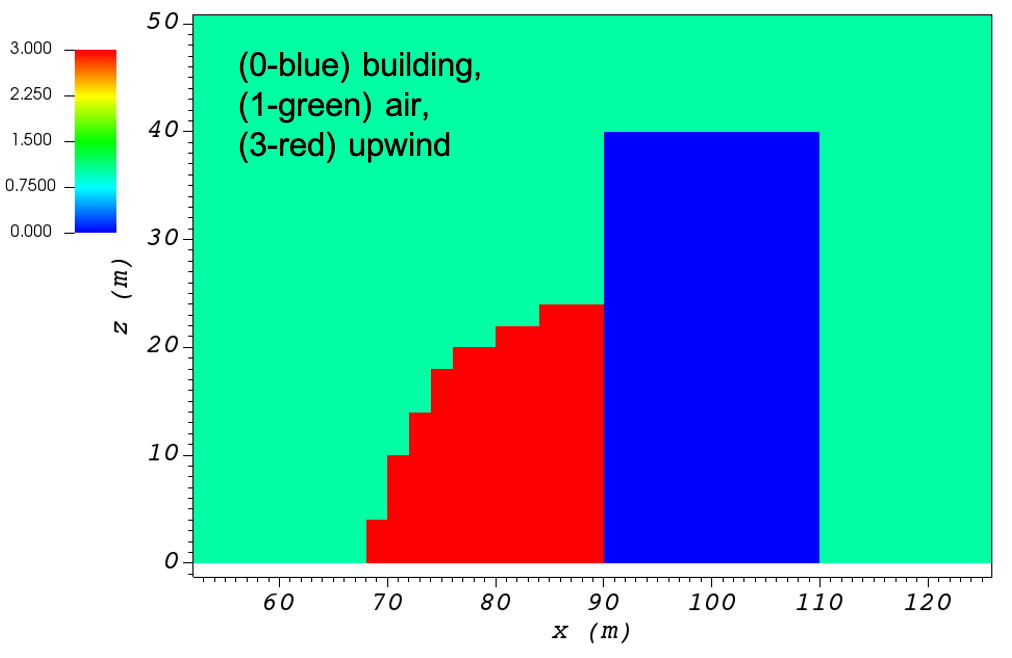
\includegraphics[width=10.3cm,keepaspectratio]{Images/upwind_y_100_2_init_icell.png}
    \caption{}
    \end{subfigure}
    \begin{subfigure}{\textwidth}
    \centering
    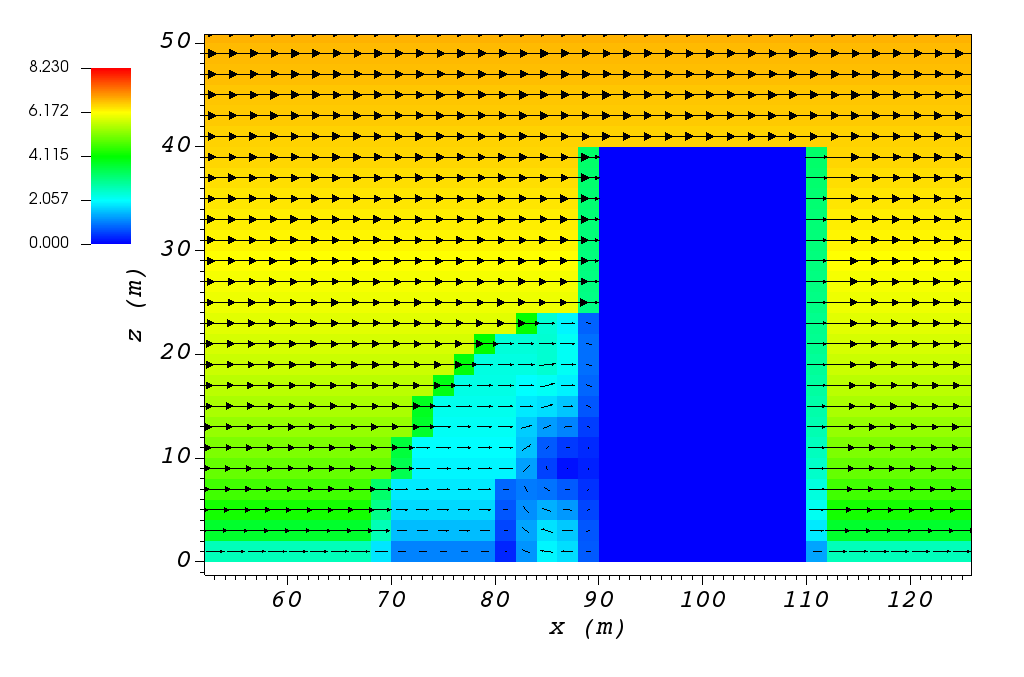
\includegraphics[width=11.0cm,keepaspectratio]{Images/upwind_y_100_2_init_vel.png}
    \caption{}
    \end{subfigure}
    \begin{subfigure}{\textwidth}
    \centering
    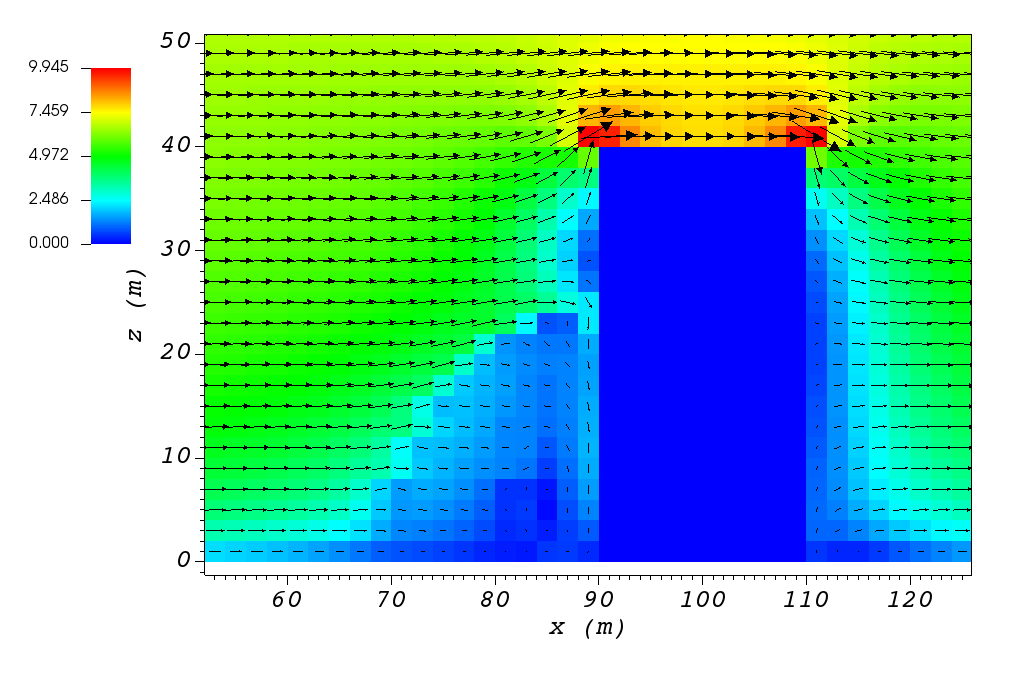
\includegraphics[width=11.0cm,keepaspectratio]{Images/upwind_y_100_2_final.png}
    \caption{}
    \end{subfigure}
    \caption{(a) Cell type contour to show the area of effect of the MVP upwind cavity parameterization in a vertical plane at $y=100$ m. Velocity magnitude contour with overlaying velocity vectors of (b) initial velocity field and (c) final velocity field, in a vertical plane at $y=100$ m.}
\end{figure}

\begin{figure}[H]
    \centering
    \begin{subfigure}{\textwidth}
    \centering
    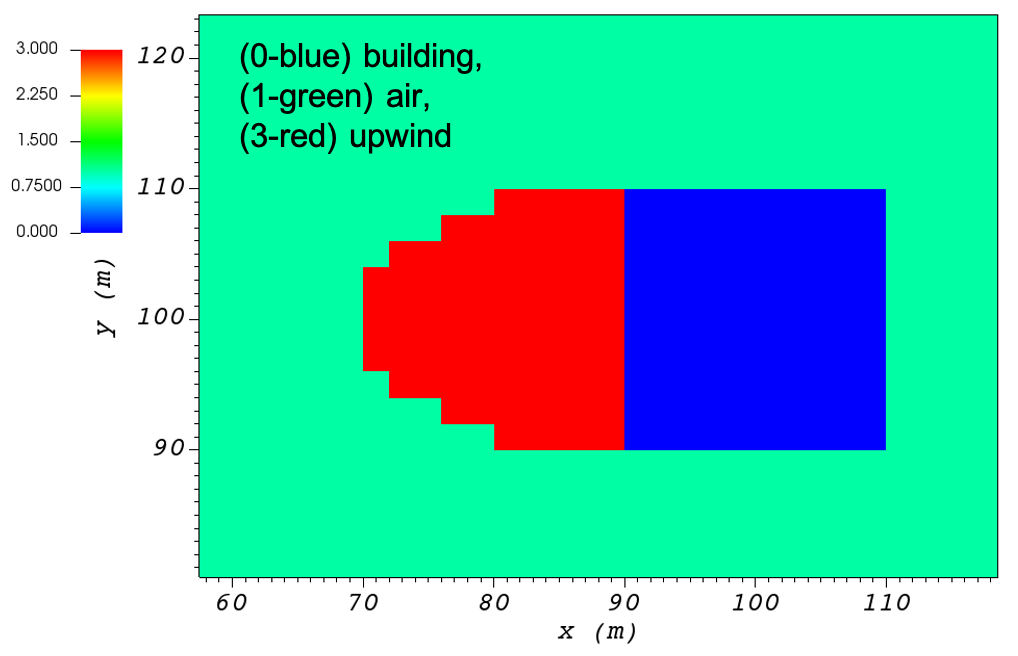
\includegraphics[width=10.3cm,keepaspectratio]{Images/upwind_z_5_2_init_icell.png}
    \caption{}
    \end{subfigure}
    \begin{subfigure}{\textwidth}
    \centering
    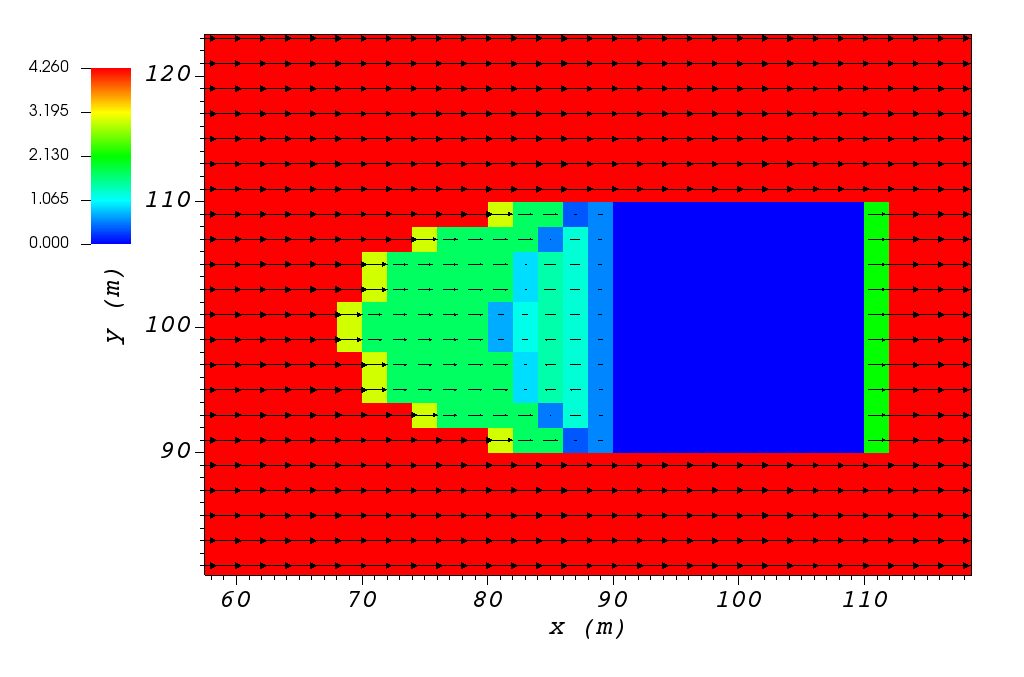
\includegraphics[width=11.0cm,keepaspectratio]{Images/upwind_z_5_2_init_vel.png}
    \caption{}
    \end{subfigure}
    \begin{subfigure}{\textwidth}
    \centering
    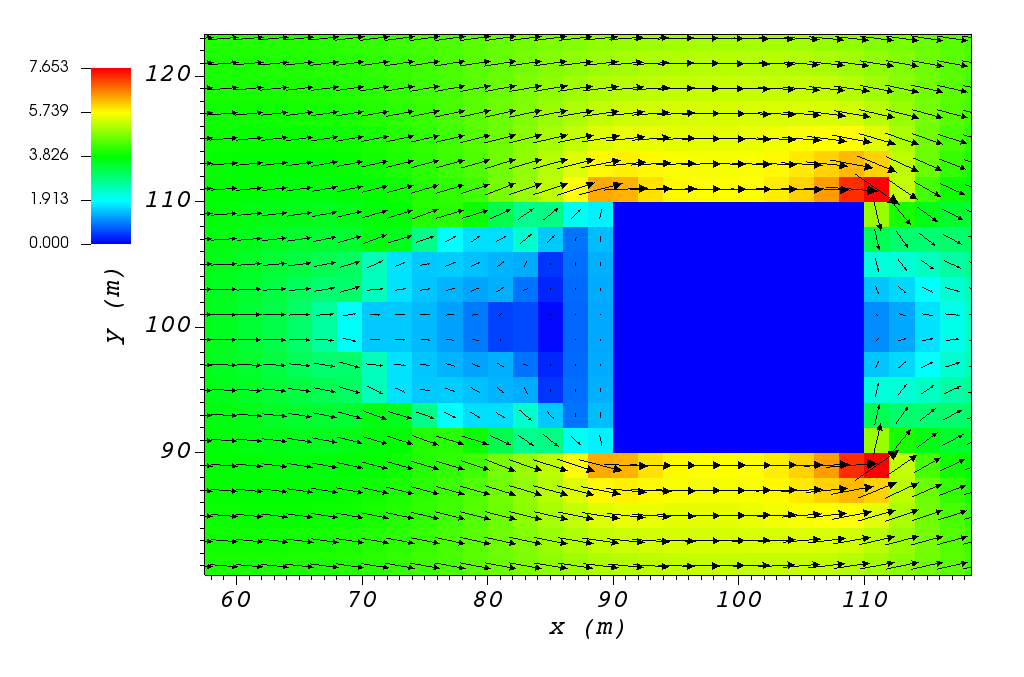
\includegraphics[width=11.0cm,keepaspectratio]{Images/upwind_z_5_2_final.png}
    \caption{}
    \end{subfigure}
    \caption{(a) Cell type contour to show the area of effect of the MVP upwind cavity parameterization in a horizontal plane at $z=5$ m. Velocity magnitude contour with overlaying velocity vectors of (b) initial velocity field and (c) final velocity field, in a horizontal plane at $z=5$ m.}
\end{figure}

The third option is called the high-rise MVP algorithm (HMVP) and is designed to address the shortcomings of the previous models when it comes to tall buildings  \cite{nelson20085}. The length of the displacement zone is calculated the same as Eq. \ref{eq:lf_MVP}. The HMVP algorithm creates two ellipsoids with the difference that the inner region only extends to $60\%$ of the minimum of building height and building width. In addition, the algorithm linearly reduces the velocities in the outer region from their upwind values at the outer surface to $40\%$ of the initial values on the inner region.

Part (a) of Figure \ref{fig:upwind_1_vert} and Figure \ref{fig:upwind_1_horiz} show cell type contour to represent the area of effect of the HMVP upwind cavity parameterization in a vertical plane at $y=100$ m and a horizontal plane at $z=5$ m, respectively. The upwind parameterization is applied to a rectangular building defined in Section \ref{sec:building}. The initial guess field is constructed using a single sensor with logarithmic profile as defined in \ref{sec:sensor_xml}. Parts (b) and (c) of Figure \ref{fig:upwind_1_vert} and Figure \ref{fig:upwind_1_horiz} indicate velocity magnitude contour with overlaying velocity vectors of initial (part (b)) and final (part(c)) velocity fields in a vertical plane at $y=100$ m and a horizontal plane at $z=5$ m, respectively.

\begin{figure}[H]
    \centering
    \begin{subfigure}{\textwidth}
    \centering
    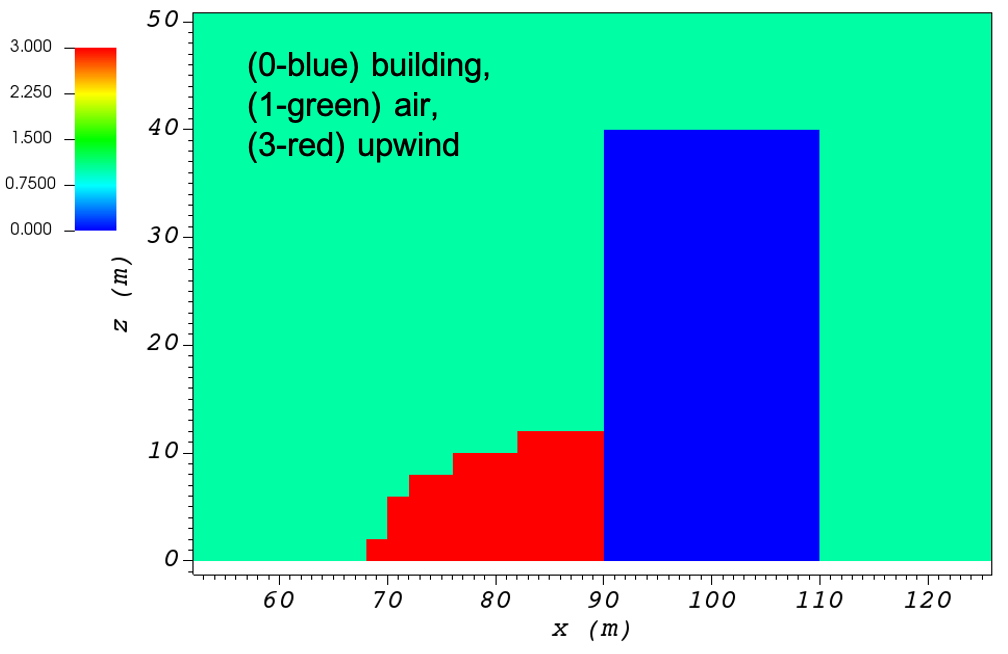
\includegraphics[width=10.3cm,keepaspectratio]{Images/upwind_y_100_3_init_icell.png}
    \caption{}
    \end{subfigure}
    \begin{subfigure}{\textwidth}
    \centering
    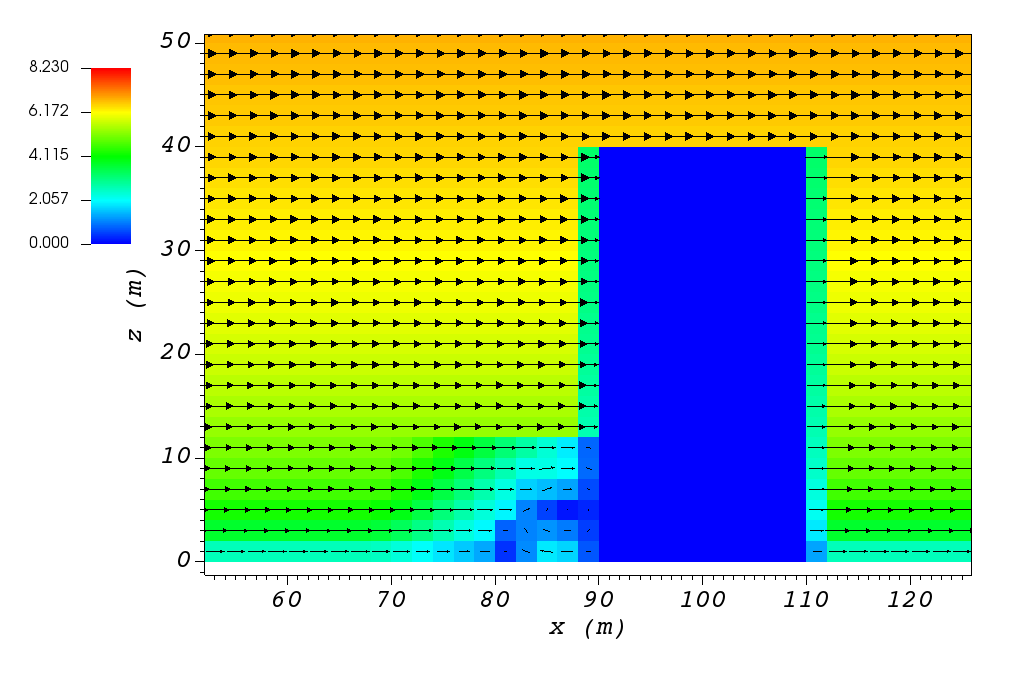
\includegraphics[width=11.0cm,keepaspectratio]{Images/upwind_y_100_3_init_vel.png}
    \caption{}
    \end{subfigure}
    \begin{subfigure}{\textwidth}
    \centering
    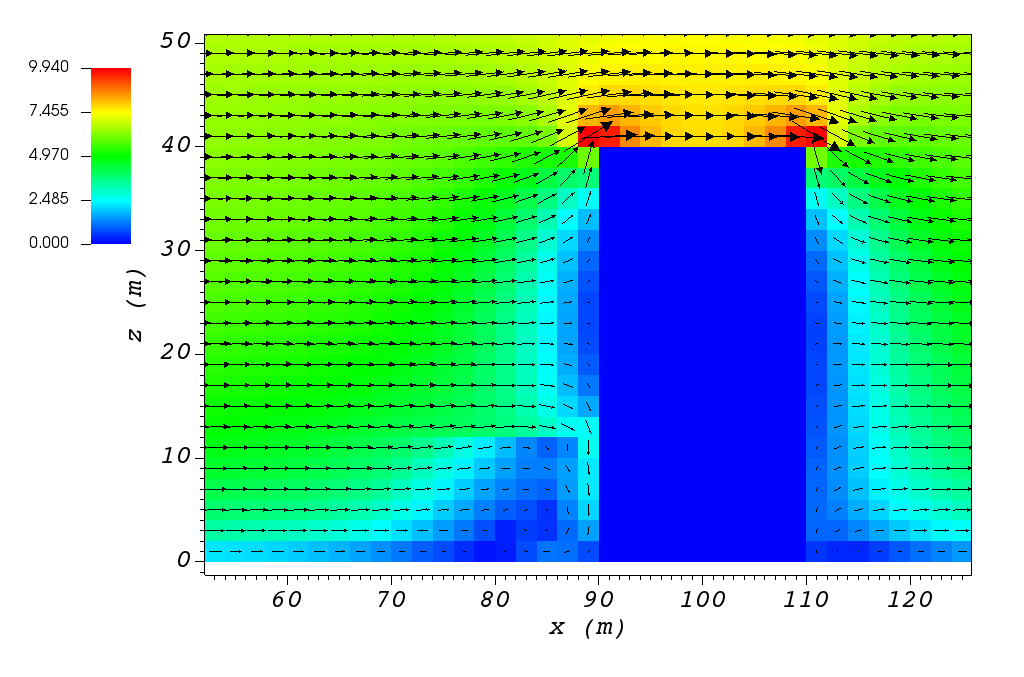
\includegraphics[width=11.0cm,keepaspectratio]{Images/upwind_y_100_3_final.png}
    \caption{}
    \end{subfigure}
    \caption{(a) Cell type contour to show the area of effect for the HMVP upwind cavity parameterization in a vertical plane at $y=100$ m. Velocity magnitude contour with overlaying velocity vectors of (b) initial velocity field and (c) final velocity field, in a vertical plane at $y=100$ m.}
\end{figure}

\begin{figure}[H]
    \centering
    \begin{subfigure}{\textwidth}
    \centering
    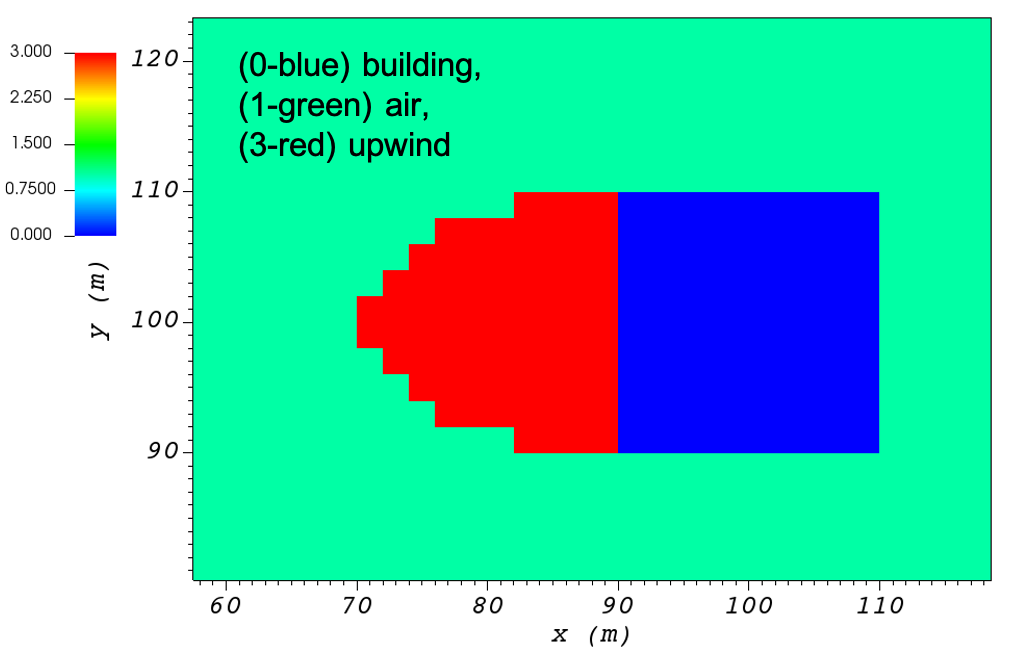
\includegraphics[width=10.3cm,keepaspectratio]{Images/upwind_z_5_3_init_icell.png}
    \caption{}
    \end{subfigure}
    \begin{subfigure}{\textwidth}
    \centering
    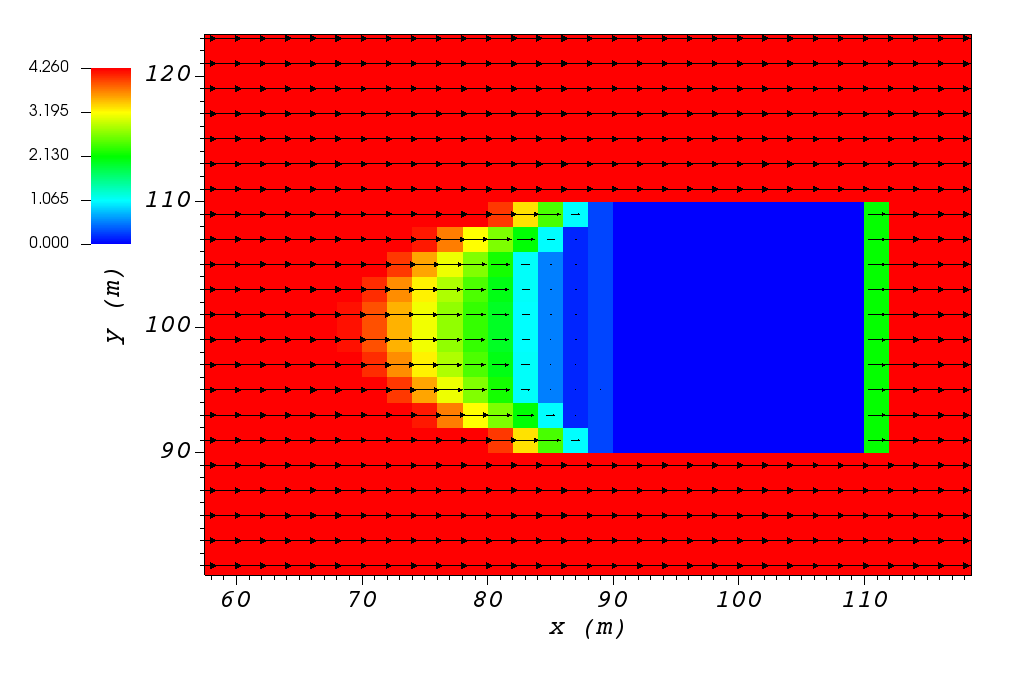
\includegraphics[width=11.0cm,keepaspectratio]{Images/upwind_z_5_3_init_vel.png}
    \caption{}
    \end{subfigure}
    \begin{subfigure}{\textwidth}
    \centering
    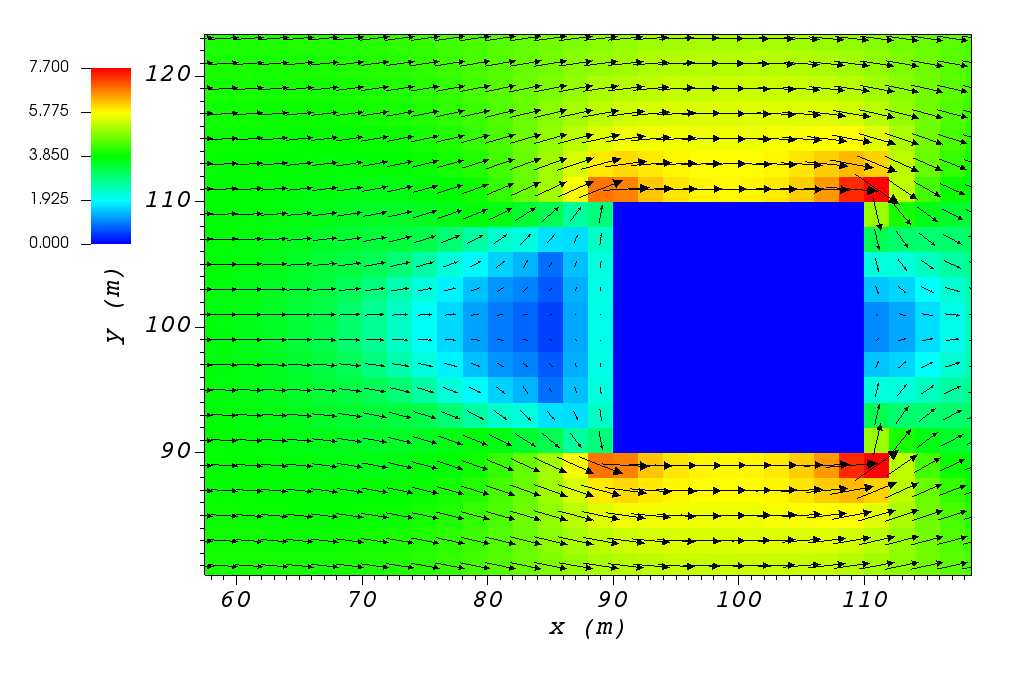
\includegraphics[width=11.0cm,keepaspectratio]{Images/upwind_z_5_3_final.png}
    \caption{}
    \end{subfigure}
    \caption{(a) Cell type contour to show the area of effect of the HMVP upwind cavity parameterization in a horizontal plane at $z=5$ m. Velocity magnitude contour with overlaying velocity vectors of (b) initial velocity field and (c) final velocity field, in a horizontal plane at $z=5$ m.}
\end{figure}

In order to choose between these three upwind models, the user needs to change the value of "upwindCavityFlag" in the XML file.


\begin{lstlisting}[language=XML]
<simulationParameters>
  	<upwindCavityFlag> 2 </upwindCavityFlag> 			<!-- Upwind cavity flag (0-none, 1-Rockle, 2-MVP (default), 3-HMVP) -->
</simulationParameters>
\end{lstlisting}

\subsection{Leeside Cavity and Far-Wake}\label{leeside-cavity-and-far-wake}

The far-wake and cavity parameterization described in \cite{singh2005testing,singh2006testing} are a significant part of the building parameterizations. The one available in QES-Winds is based on the parameterization proposed by R\"{o}ckle \cite{rockle1990bestimmung} and later Kaplan and Dinar \cite{kaplan1996lagrangian}. The R\"{o}ckle parameterization defines two ellipsoids to represent the shape of the reversed flow cavity and the far-wake region. The reversed flow cavity extends to the along-wind cavity length
($L_R$), which is calculated as:
\begin{equation}
\frac{L_{R}}{H}=\frac{1.8 \frac{W}{H}}{\left(\frac{L}{H}\right)^{0.3}\left(1+0.24 \frac{W}{H}\right)},
\label{eq:Lr}
\end{equation}
and wake is assumed to be approximately $3$ cavity lengths long (i.e., $3L_R$). After calculating $L_R$, the cavity length, $d$ in the stream-wise direction was defined by an ellipsoid shape using: 
\begin{equation}
d=L_{R} \sqrt{\left(1-\left(\frac{z}{H}\right)^{2}\right)\left(1-\left(\frac{y}{W}\right)^{2}\right)}-\frac{L}{2}.
\label{eq:d}
\end{equation} 
Finally, the velocity in the reversed cavity zone is defined using:
\begin{equation}
\frac{u(x, y, z)}{U(H)}=-\left(1-\left(\frac{x}{d}\right)^{2}\right)
\label{eq:cavity}
\end{equation}
and in the wake region, the velocity field is estimated by: 
\begin{equation}
\frac{u(x, y, z)}{U(H)}=\left(1-\left(\frac{d}{x}\right)^{1.5}\right).
\label{eq:wake}
\end{equation}

where $L$, $H$ and $W$ are length, width and height of the building, receptively. $u(x,y,z)$ is the velocity at point $(x,y,z)$, $U(H)$ is the reference velocity at height of the building and $x$ is the distance from the building in the stream-wise direction.

Part (a) of Figure \ref{fig:wake_vert} and Figure \ref{fig:wake_horiz} show cell type contour to represent the area of effect of the R\"{o}ckle wake parameterization in a vertical plane at $y=100$ m and a horizontal plane at $z=5$ m, respectively. The wake parameterization is applied to a rectangular building defined in Section \ref{sec:building}. The initial guess field is constructed using a single sensor with logarithmic profile as defined in \ref{sec:sensor_xml}. Parts (b) and (c) of Figure \ref{fig:wake_vert} and Figure \ref{fig:wake_horiz} indicate velocity magnitude contour with overlaying velocity vectors of initial (part (b)) and final (part(c)) velocity fields in a vertical plane at $y=100$ m and a horizontal plane at $z=5$ m, respectively.

\begin{figure}[H]
    \centering
    \begin{subfigure}{\textwidth}
    \centering
    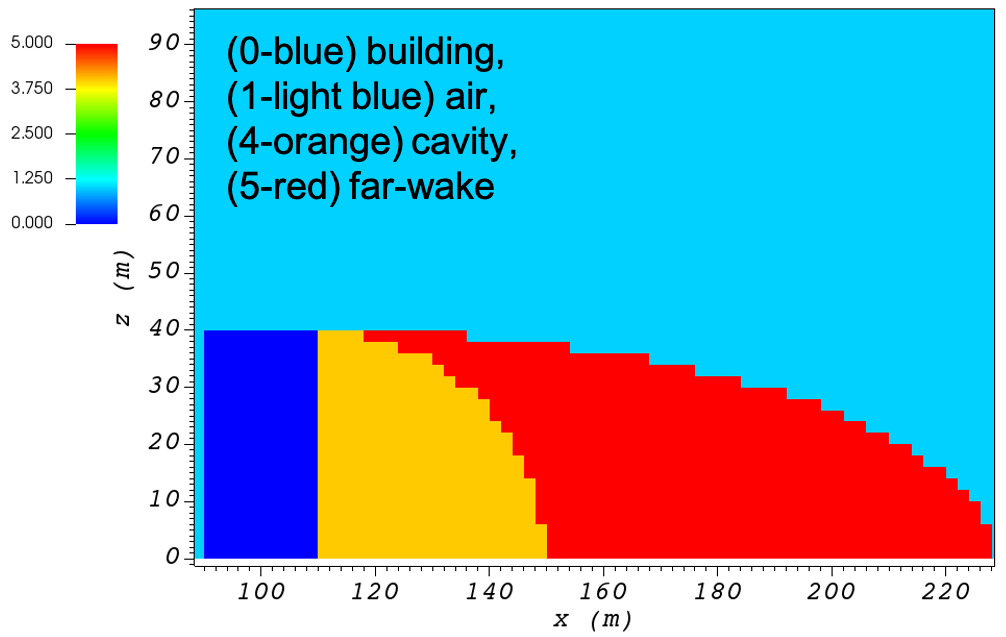
\includegraphics[width=10.3cm,keepaspectratio]{Images/wake_y_100_1_init_icell.png}
    \caption{}
    \end{subfigure}
    \begin{subfigure}{\textwidth}
    \centering
    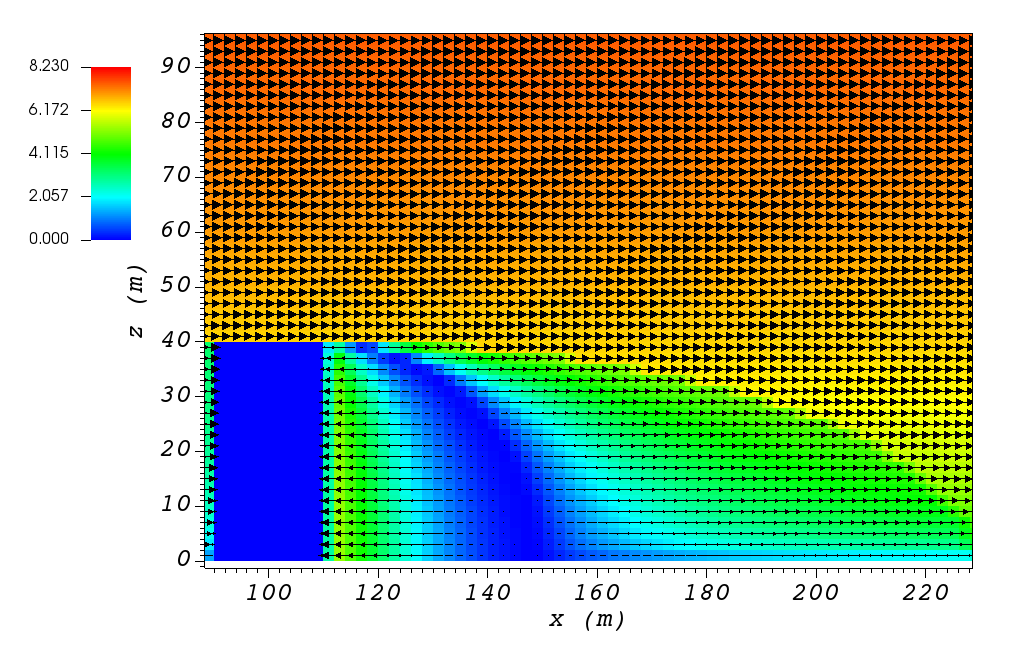
\includegraphics[width=11.0cm,keepaspectratio]{Images/wake_y_100_1_init_vel.png}
    \caption{}
    \end{subfigure}
    \begin{subfigure}{\textwidth}
    \centering
    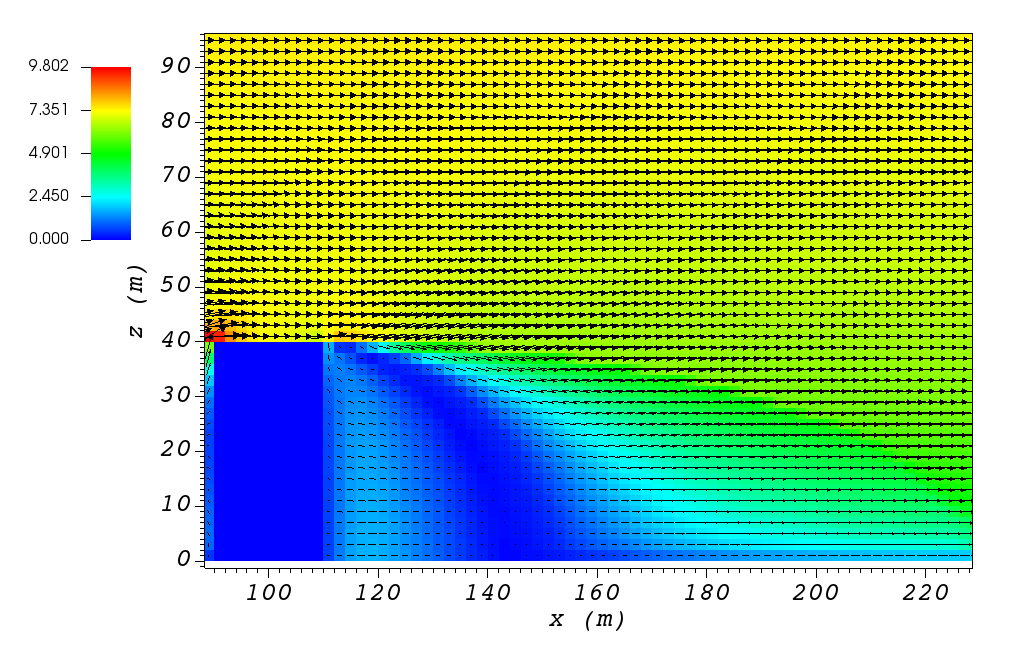
\includegraphics[width=11.0cm,keepaspectratio]{Images/wake_y_100_1_final.png}
    \caption{}
    \end{subfigure}
    \caption{(a) Cell type contour to show the area of effect of the R\"{o}ckle wake parameterization in a vertical plane at $y=100$ m. Velocity magnitude contour with overlaying velocity vectors of (b) initial velocity field and (c) final velocity field, in a vertical plane at $y=100$ m.}
\end{figure}

\begin{figure}[H]
    \centering
    \begin{subfigure}{\textwidth}
    \centering
    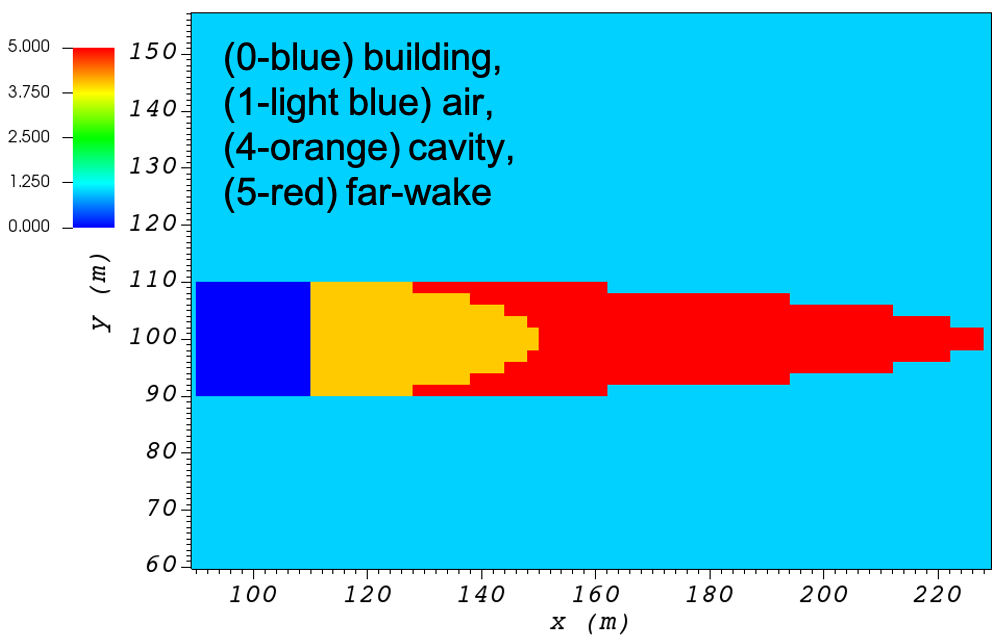
\includegraphics[width=10.3cm,keepaspectratio]{Images/wake_z_5_1_init_icell.png}
    \caption{}
    \end{subfigure}
    \begin{subfigure}{\textwidth}
    \centering
    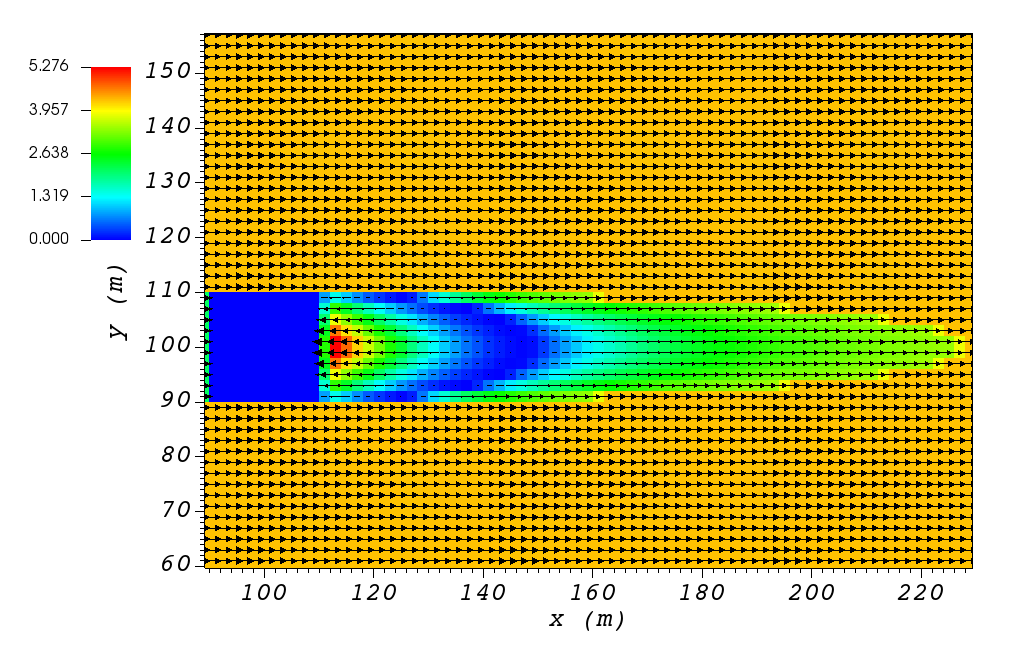
\includegraphics[width=11.0cm,keepaspectratio]{Images/wake_z_5_1_init_vel.png}
    \caption{}
    \end{subfigure}
    \begin{subfigure}{\textwidth}
    \centering
    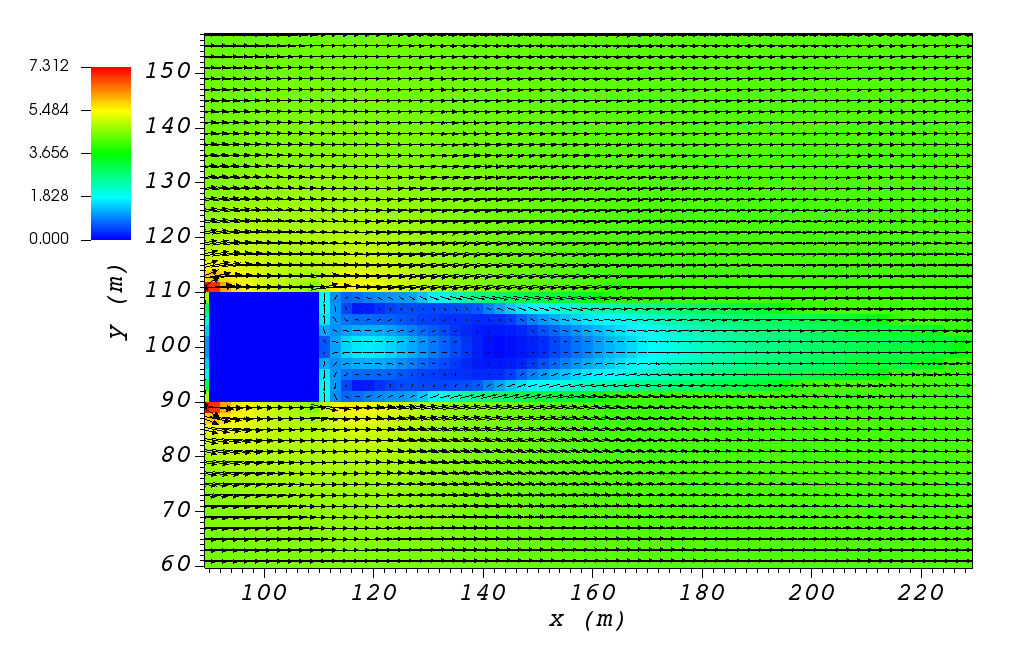
\includegraphics[width=11.0cm,keepaspectratio]{Images/wake_z_5_1_final.png}
    \caption{}
    \end{subfigure}
    \caption{(a) Cell type contour to show the area of effect of the R\"{o}ckle wake parameterization in a horizontal plane at $z=5$ m. Velocity magnitude contour with overlaying velocity vectors of (b) initial velocity field and (c) final velocity field, in a horizontal plane at $z=5$ m.}
\end{figure}

In order to turn on the wake model, the user needs to change the value of "wakeFlag" in the XML file.

\begin{lstlisting}[language=XML]
<simulationParameters>
  	<wakeFlag> 1 </wakeFlag> 				<!-- Wake flag (0-none, 1-Rockle (default)) -->
</simulationParameters>
\end{lstlisting}

\subsection{Street Canyon}

The street canyon parameterization detailed in \cite{singh2008evaluation} represents the effects of two buildings in close vicinity to each other, on the fluid flow. R\"{o}ckle \cite{rockle1990bestimmung} introduced velocity parameterizations for the stream-wise components as: 
\begin{equation}
\frac{u(x, y, z)}{U(H)}=-\frac{x_{\mathrm{can}}}{(0.5 S)}\left(\frac{S-x_{\mathrm{can}}}{0.5 S}\right)
\label{eq:u_can}
\end{equation}
and the vertical component as 
\begin{equation}
\frac{w(x, y, z)}{U(H)}=-\left|\frac{1}{2}\left(1-\frac{x_{\text {can }}}{0.5 S}\right)\right|\left(1-\frac{S-x_{\text {can }}}{0.5 S}\right).
\label{eq:w_can}
\end{equation}

where $S$ is the spacing between two buildings and $x_{can}$ is the distance from the backwall of the upwind building.

In order to identify the criteria to determine the existence of a street canyon, Singh et al. \cite{singh2008evaluation} utilized the cavity length, $L_R$ (Eq. \ref{eq:Lr}), for the upwind building. If $S \textless L_R$, the street canyon parameterization is applied, otherwise, the upwind building is considered as an isolated building.

Part (a) of Figure \ref{fig:street_vert} and Figure \ref{fig:street_horiz} show cell type contour to represent the area of effect of the street canyon parameterization in a vertical plane at $y=100$ m and a horizontal plane at $z=5$ m, respectively. The street canyon parameterization is applied to an area between two rectangular buildings. The upwind building is same as the one defined in Section \ref{sec:building}. The downwind building is a rectangular building with $20$ m as height, $0$ m as base height, $20$ m as length and width, closest corner to the origin located at $90$ m in $x$ and $120$ m in $y$ directions, and $0^{\circ}$ as rotation angle with respect to the North-South line. The initial guess field is constructed using a single sensor with logarithmic profile as defined in \ref{sec:sensor_xml}. Parts (b) and (c) of Figure \ref{fig:street_vert} and Figure \ref{fig:street_horiz} indicate velocity magnitude contour with overlaying velocity vectors of initial (part (b)) and final (part(c)) velocity fields in a vertical plane at $y=100$ m and a horizontal plane at $z=5$ m, respectively.

\begin{figure}[H]
    \centering
    \begin{subfigure}{\textwidth}
    \centering
    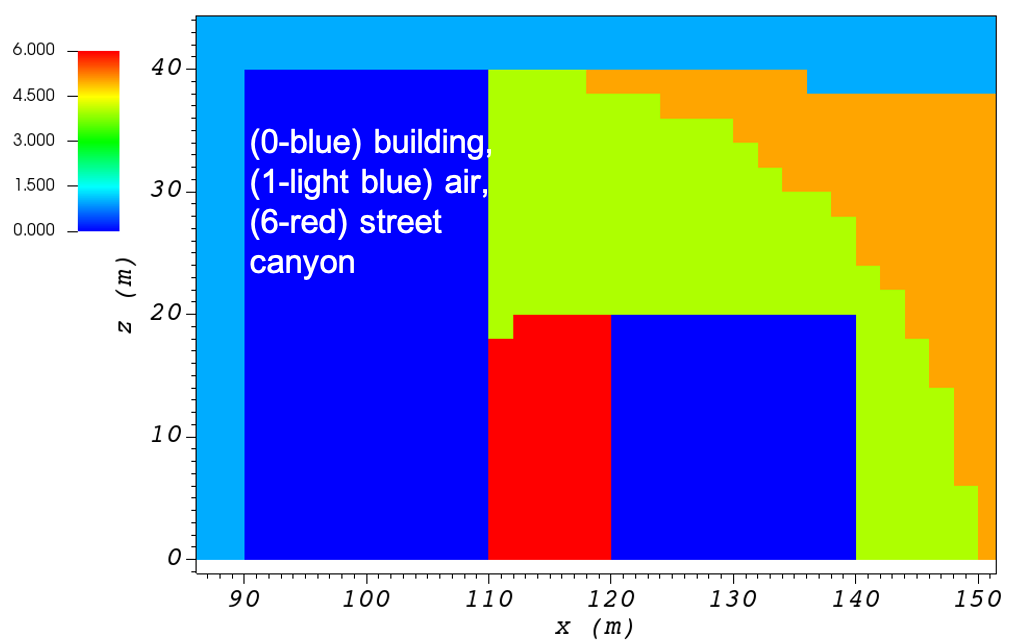
\includegraphics[width=10.3cm,keepaspectratio]{Images/street_y_100_1_init_icell.png}
    \caption{}
    \end{subfigure}
    \begin{subfigure}{\textwidth}
    \centering
    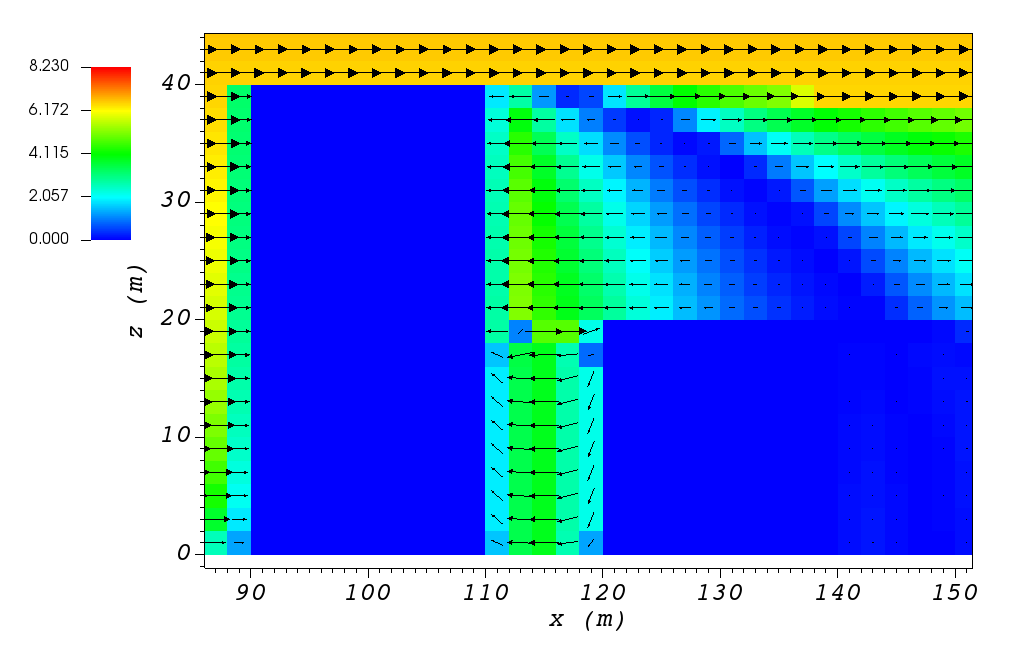
\includegraphics[width=11.0cm,keepaspectratio]{Images/street_y_100_1_init_vel.png}
    \caption{}
    \end{subfigure}
    \begin{subfigure}{\textwidth}
    \centering
    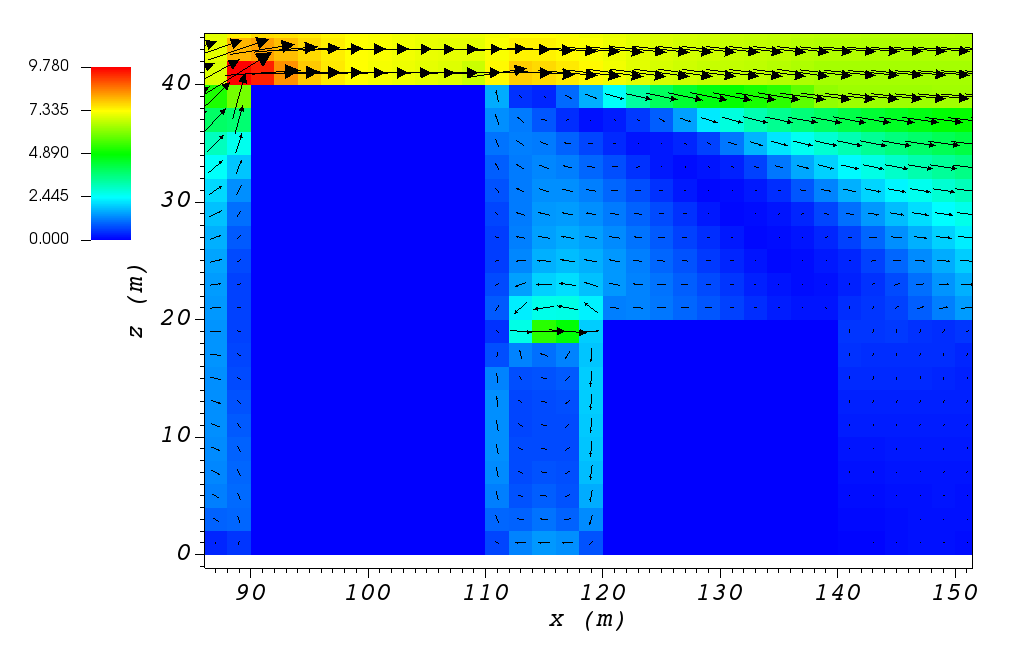
\includegraphics[width=11.0cm,keepaspectratio]{Images/street_y_100_1_final.png}
    \caption{}
    \end{subfigure}
    \caption{(a) Cell type contour to show the area of effect of the street canyon parameterization in a vertical plane at $y=100$ m. Velocity magnitude contour with overlaying velocity vectors of (b) initial velocity field and (c) final velocity field, in a vertical plane at $y=100$ m.}
\end{figure}

\begin{figure}[H]
    \centering
    \begin{subfigure}{\textwidth}
    \centering
    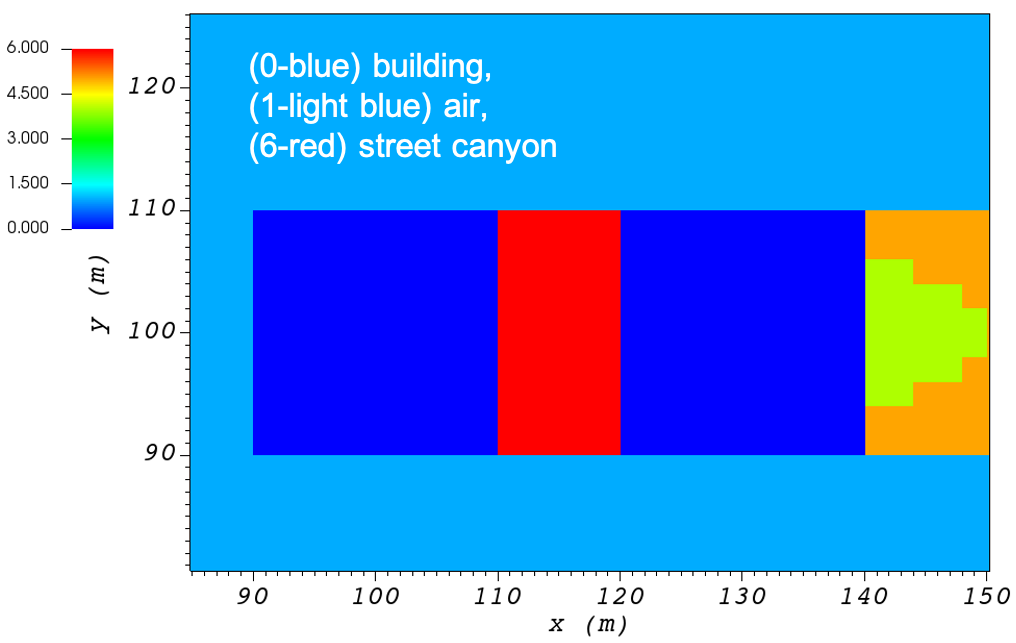
\includegraphics[width=10.3cm,keepaspectratio]{Images/street_z_5_1_init_icell.png}
    \caption{}
    \end{subfigure}
    \begin{subfigure}{\textwidth}
    \centering
    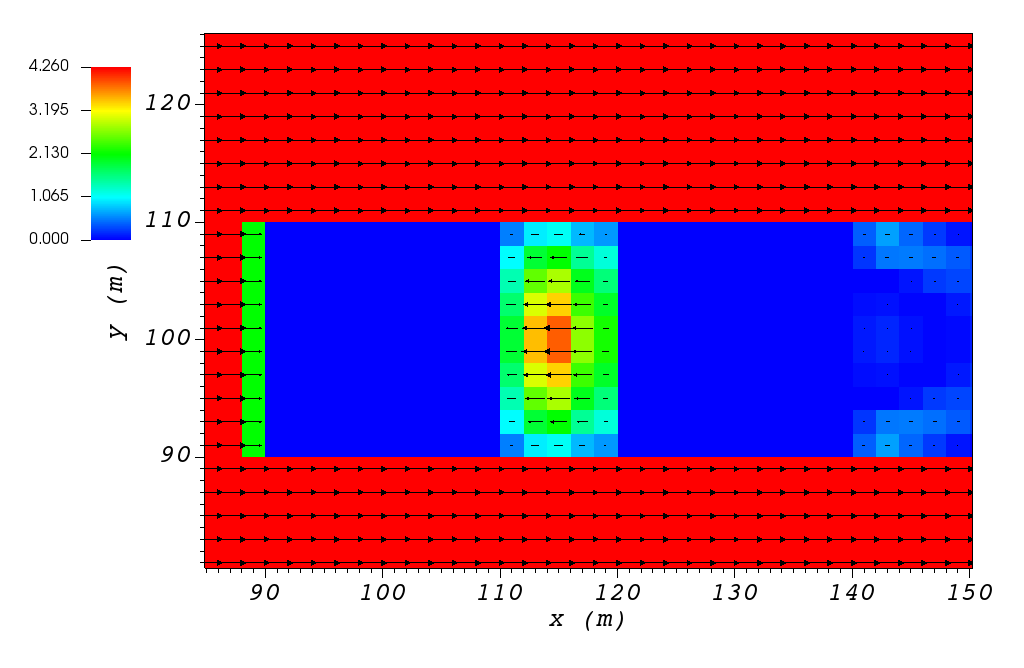
\includegraphics[width=11.0cm,keepaspectratio]{Images/street_z_5_1_init_vel.png}
    \caption{}
    \end{subfigure}
    \begin{subfigure}{\textwidth}
    \centering
    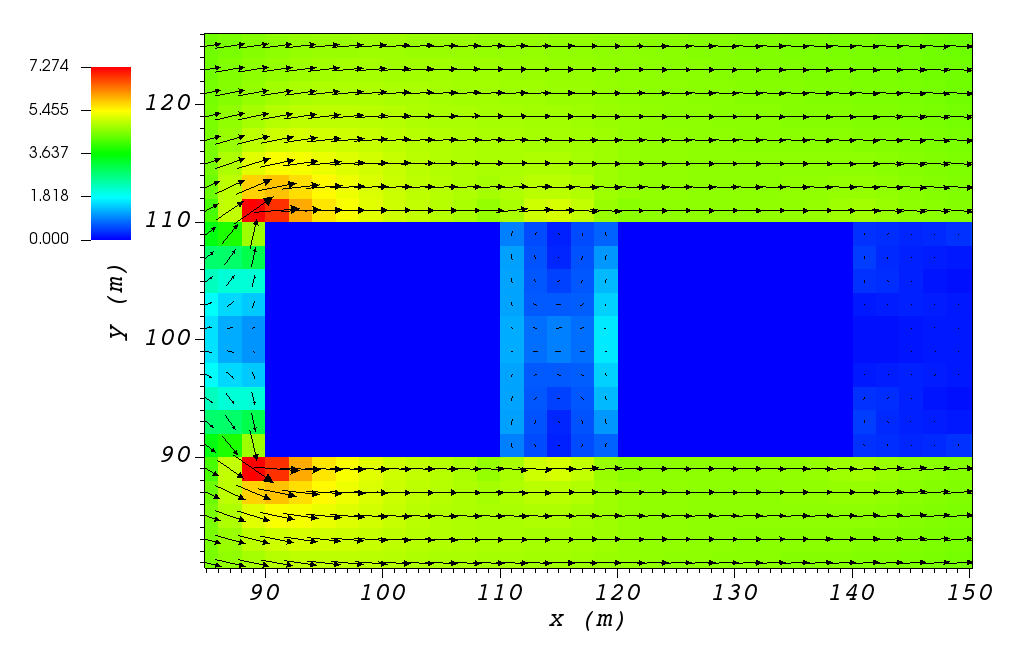
\includegraphics[width=11.0cm,keepaspectratio]{Images/street_z_5_1_final.png}
    \caption{}
    \end{subfigure}
    \caption{(a) Cell type contour to show the area of effect of the street canyon parameterization in a horizontal plane at $z=5$ m. Velocity magnitude contour with overlaying velocity vectors of (b) initial velocity field and (c) final velocity field, in a horizontal plane at $z=5$ m.}
\end{figure}

To turn on the street canyon parameterization, the user needs to change the value of "streetCanyonFlag" in the XML file.

\begin{lstlisting}[language=XML]
<simulationParameters>
  	<streetCanyonFlag> 1 </streetCanyonFlag> 			<!-- Street canyon flag (0-none, 1-Roeckle w/ Fackrel (default)) -->
</simulationParameters>
\end{lstlisting}

\subsection{Rooftop Recirculation}

The rooftop parameterization described in \cite{bagal2004implementation,pol2006implementation}, captures the separation of the flow from the leading edge of the building. It first checks if the incident flow is in $\pm15^{\circ}$ of perpendicular to the front face. The parameterization then creates an ellipsoidal region above the building with height of $H_c$ (height of the vortex, calculated by Eq. \ref{eq:Hc}) and length of $L_c$ (length of the vortex, calculated by Eq. \ref{eq:Lc}). It applies a logarithmic profile in the whole vortex area and finally, reverses the velocity in region $1$. Region $1$ is an ellipsoidal zone with the same length as the vortex and half of the height.

\begin{equation}
R=B_{\mathrm{s}}^{2 / 3} B_{l}^{1 / 3}
\end{equation}

\begin{equation}
L_{\mathrm{c}}=0.9 R
\label{eq:Lc}
\end{equation}

\begin{equation}
H_{\mathrm{c}}=0.22 R
\label{eq:Hc}
\end{equation}

where $B_s$ is the smaller of the height ($H$) and the effective width ($W_{eff}$) of the
building, $B_l$ is the larger of $H$ and $W_{eff}$ , $R$ is the vortex size scaling factor.

Part (a) of Figure \ref{fig:street_vert} show cell type contour to represent the area of effect of the rooftop parameterization in a vertical plane at $y=100$ m. The rooftop parameterization is applied to a rectangular building with $40$ m as height, $0$ m as base height, $40$ m as length and width, closest corner to the origin located at $90$ m in $x$ and $y$ directions, and $0^{\circ}$ as rotation angle with respect to the North-South line. The initial guess field is constructed using a single sensor with logarithmic profile as defined in \ref{sec:sensor_xml}. Parts (b) and (c) of Figure \ref{fig:street_vert} indicate velocity magnitude contour with overlaying velocity vectors of initial (part (b)) and final (part(c)) velocity fields in a vertical plane at $y=100$ m.

\begin{figure}[H]
    \centering
    \begin{subfigure}{\textwidth}
    \centering
    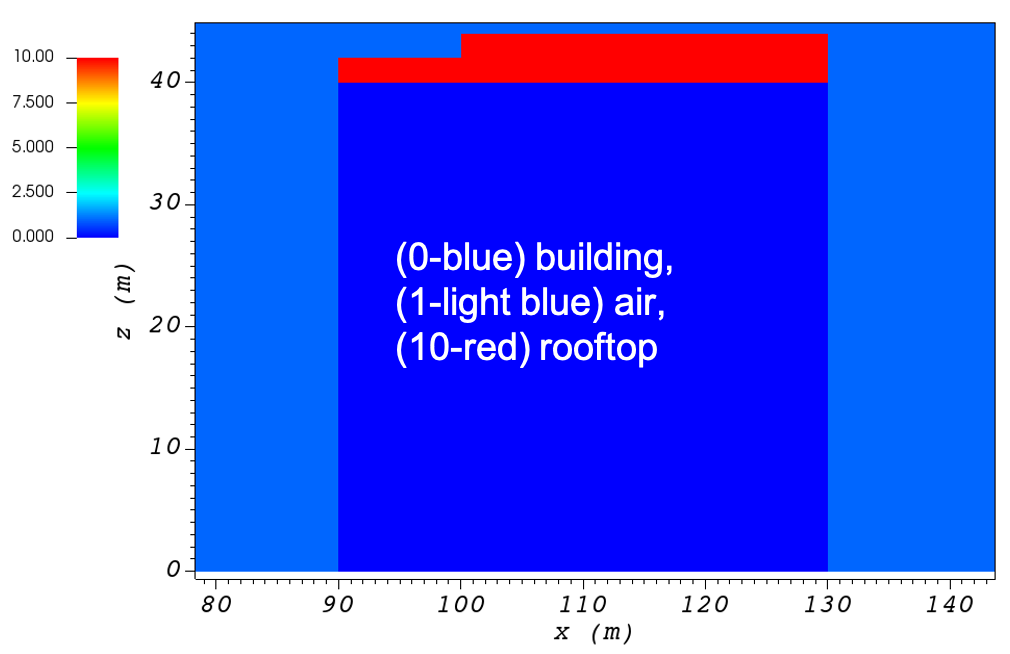
\includegraphics[width=10.3cm,keepaspectratio]{Images/rooftop_y_100_1_init_icell.png}
    \caption{}
    \end{subfigure}
    \begin{subfigure}{\textwidth}
    \centering
    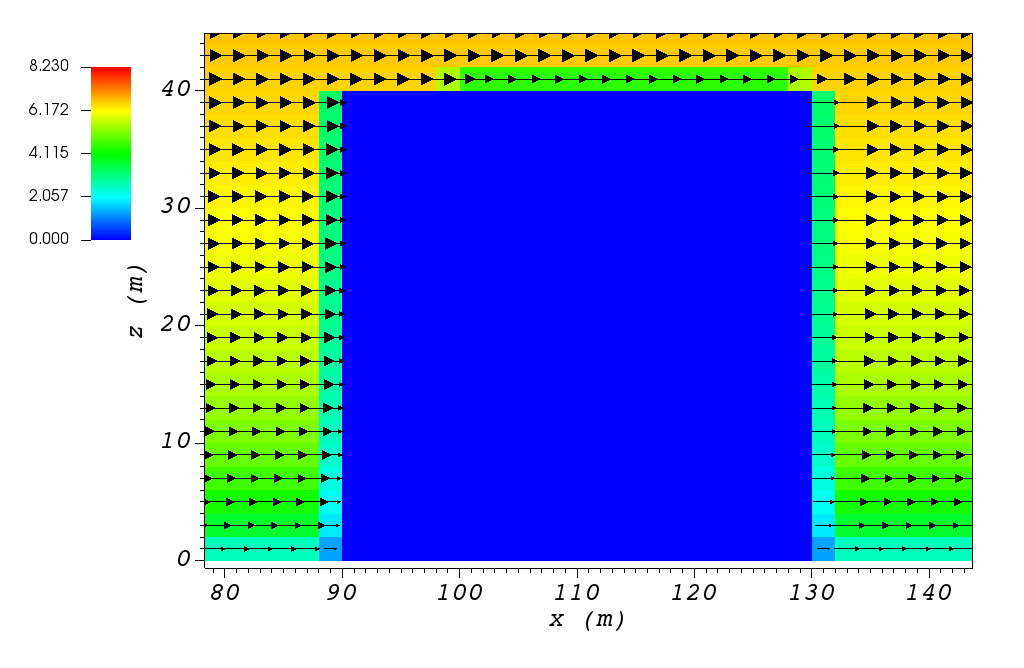
\includegraphics[width=11.0cm,keepaspectratio]{Images/rooftop_y_100_1_init_vel.png}
    \caption{}
    \end{subfigure}
    \begin{subfigure}{\textwidth}
    \centering
    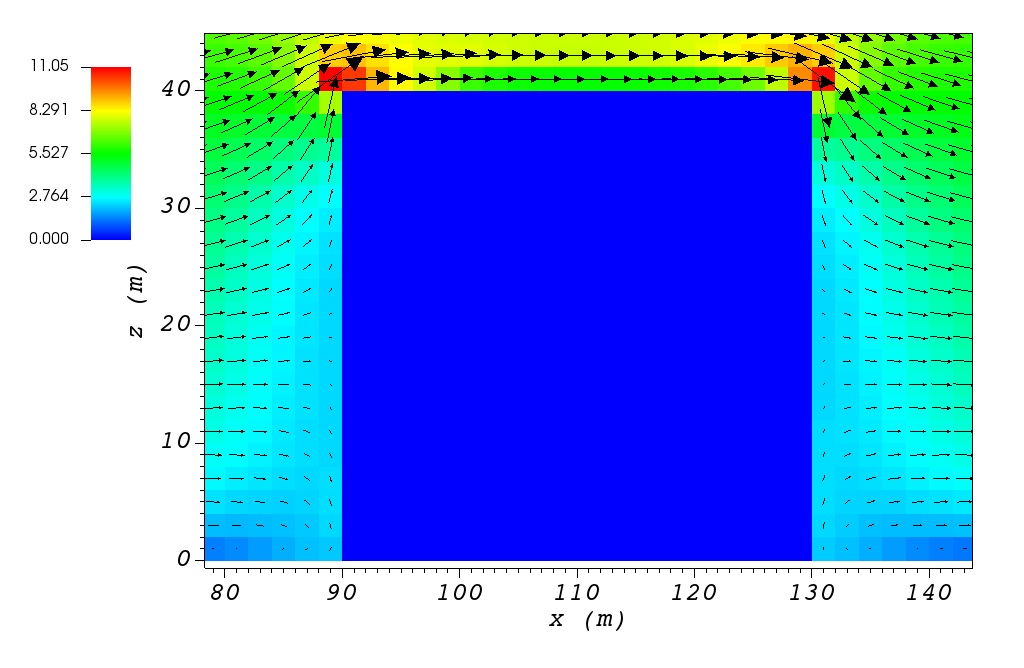
\includegraphics[width=11.0cm,keepaspectratio]{Images/rooftop_y_100_1_final.png}
    \caption{}
    \end{subfigure}
    \caption{(a) Cell type contour to show the area of effect of the rooftop parameterization in a vertical plane at $y=100$ m. Velocity magnitude contour with overlaying velocity vectors of (b) initial velocity field and (c) final velocity field, in a vertical plane at $y=100$ m.}
\end{figure}

To turn the parameterization on, the user needs to change the value of "rooftopFlag" in the XML file.

\begin{lstlisting}[language=XML]
<simulationParameters>
  	<rooftopFlag> 1 </rooftopFlag> 					<!-- Rooftop flag (0-none, 1-log profile (default)) -->
</simulationParameters>
\end{lstlisting}

\subsection{Sidewall Recirculation Zone}

The sidewall parameterization is designed to represent the effects of the edge of the building on the upwind field \cite{hayati2017comprehensive}. It first checks if a face has an outward normal vector nominally ($\pm 10^{\circ}$)
perpendicular to the local wind vector. The important parameters controlling the sidewall vortex strength and geometry are:

\begin{equation}
R=B_{\mathrm{s}}^{2 / 3} B_{l}^{1 / 3}
\end{equation}

\begin{equation}
L_{\mathrm{c}}=0.9 R
\end{equation}

\begin{equation}
W_{\mathrm{c}}=0.22 R
\end{equation}

where $B_s$ is the smaller of the height ($H$) and the effective width ($W_{eff}$) of the
building, $B_l$ is the larger of $H$ and $W_{eff}$ , $R$ is the vortex size scaling factor, $L_c$ is the downwind length of the half-ellipse that defines the vortex recirculation region, and
$W_c$ is the lateral width of the elliptical recirculation region. Within the recirculation zone, the velocity is reversed and scaled linearly from the reference wind speed near the wall to zero at the edge of the ellipse.

Part (a) of Figure \ref{fig:street_vert} show cell type contour to represent the area of effect of the sidewall parameterization in a horizontal plane at $z=5$ m. The rooftop parameterization is applied to a rectangular building defined in Section \ref{sec:building}. The initial guess field is constructed using a single sensor with logarithmic profile as defined in \ref{sec:sensor_xml}. Parts (b) and (c) of Figure \ref{fig:sidewall_horiz} indicate velocity magnitude contour with overlaying velocity vectors of initial (part (b)) and final (part(c)) velocity fields in a horizontal plane at $z=5$ m.

\begin{figure}[H]
    \centering
    \begin{subfigure}{\textwidth}
    \centering
    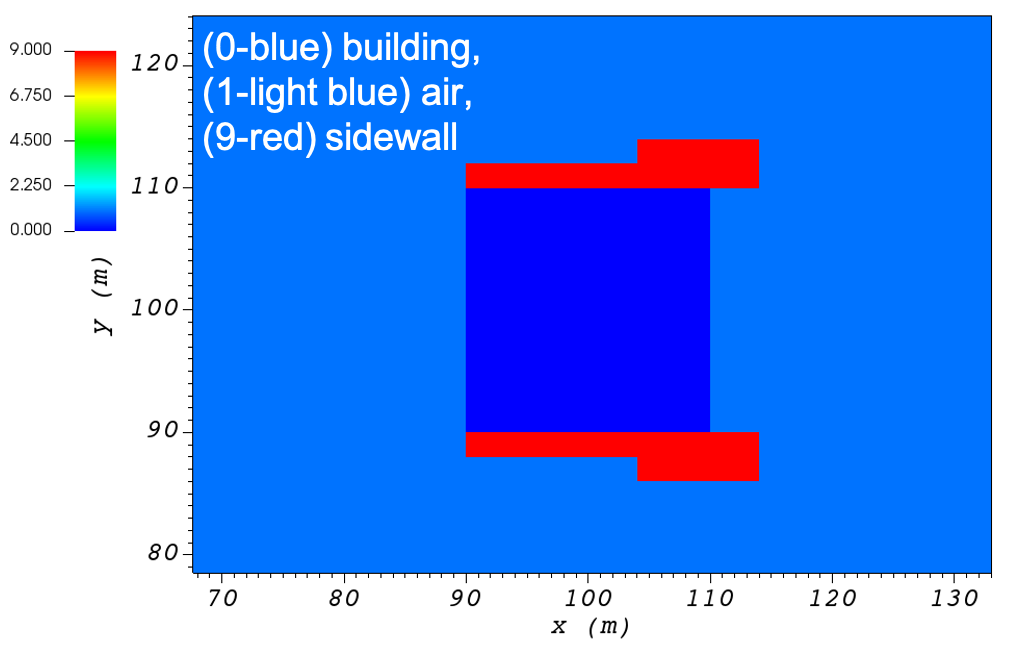
\includegraphics[width=10.3cm,keepaspectratio]{Images/sidewall_z_5_1_init_icell.png}
    \caption{}
    \end{subfigure}
    \begin{subfigure}{\textwidth}
    \centering
    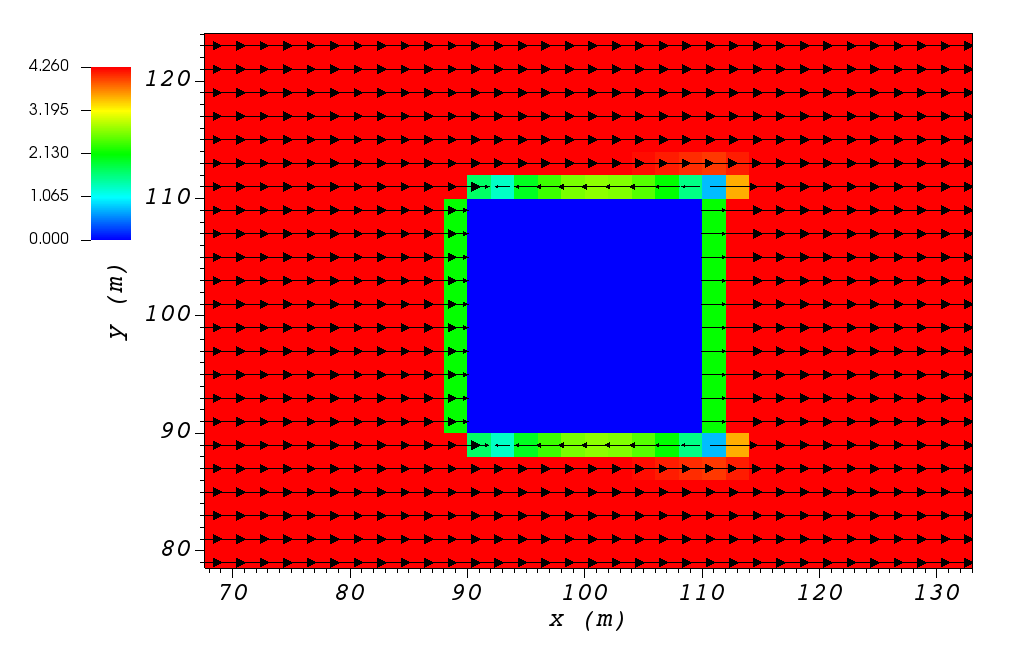
\includegraphics[width=11.0cm,keepaspectratio]{Images/sidewall_z_5_1_init_vel.png}
    \caption{}
    \end{subfigure}
    \begin{subfigure}{\textwidth}
    \centering
    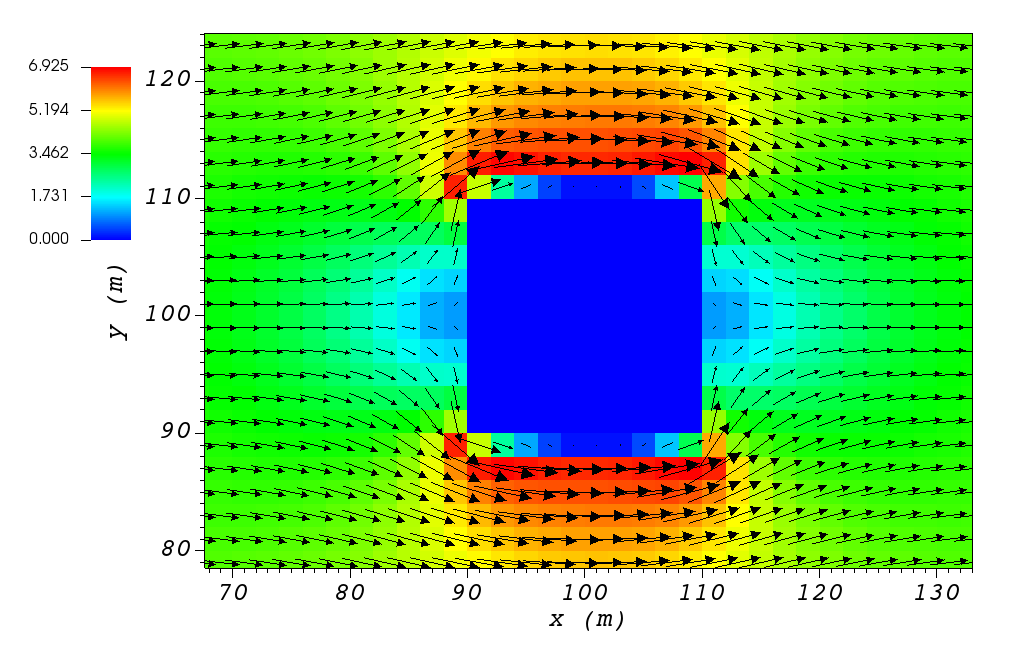
\includegraphics[width=11.0cm,keepaspectratio]{Images/sidewall_z_5_1_final.png}
    \caption{}
    \end{subfigure}
    \caption{(a) Cell type contour to show the area of effect of the sidewall parameterization in a horizontal plane at $z=5$ m. Velocity magnitude contour with overlaying velocity vectors of (b) initial velocity field and (c) final velocity field, in a horizontal plane at $z=5$ m.}
\end{figure}

In order to turn the algorithm on, the user needs to change the value of "sidewallFlag" in the XML file.

\begin{lstlisting}[language=XML]
<simulationParameters>
  	<sidewallFlag> 1 </sidewallFlag> 				<!-- Sidewall flag (0-off, 1-on (default)) -->
</simulationParameters>
\end{lstlisting}

\section{Mass Consistent Solver}

QES-Winds have mass conserving wind field solvers that rapidly compute wind fields using a variational method rather than slower yet more physics based solvers that include conservation of momentum \cite{kim2014effects}. While the QES-Winds method uses reduced order physics in the numerical solution of urban flow problems, the solutions are rapid and compare quite well higher order physics-based models in both idealized \cite{hayati2017comprehensive} and realistic urban cities \cite{neophytou2011inter}. The method minimizes the difference between an initial wind field that is specified using empirical parameterizations \cite{singh2008evaluation} and the final wind fields. The empirical parameterizations account for complex wind fields around buildings such as wake cavities downstream of a building. To obtain a quasi-time-averaged velocity field, QES-Winds uses a variational analysis technique \cite{singh2008evaluation}. This method requires the solution of a Poisson equation for Lagrange multipliers, $\lambda$ (Equation \ref{poisson}) in the following form:

\begin{equation} \label{poisson}
\frac{\partial^2\lambda}{\partial x^2} + \frac{\partial^2\lambda}{\partial y^2} + (\frac{\alpha_1}{\alpha_2})^2\:  \frac{\partial^2\lambda}{\partial z^2} = R
\end{equation}

Where R is divergence of the initial wind field and is defined as:

\begin{equation} \label{divergence}
 R = -2\,\alpha_1^2\,\Bigg[\frac{u_{i+1/2}^0-u_{i-1/2}^0}{\Delta x} + \frac{v_{j+1/2}^0-v_{j-1/2}^0}{\Delta y} + \frac{w_{k+1/2}^0-w_{k-1/2}^0}{\Delta z}\Bigg]
\end{equation}

The final velocity field is updated using Euler-Lagrange equations:

 \begin{equation} \label{eu-lag1}
 u = u^0 + \frac{1}{2\,\alpha_1^2\,\Delta x}\,[\lambda_{i+1\,,j,\,k}-\lambda_{i,\,j,\,k}]
\end{equation}

\begin{equation}
\label{eu-lag2}
 v = v^0 + \frac{1}{2\,\alpha_1^2\,\Delta y}\,[\lambda_{i,\,j+1,\,k}-\lambda_{i,\,j,\,k}]
\end{equation}

\begin{equation}
\label{eu-lag3}
 w = w^0 + \frac{1}{2\,\alpha_2^2\,\Delta z}\,[\lambda_{i,\,j,\,k+1}-\lambda_{i,\,j,\,k}]
\end{equation}

The Poisson equation is solved using the Successive Over-Relaxation (SOR) method which is a variant of Gauss-Seidel method with faster convergence. Applying SOR to Equation \ref{poisson} results in:
\begin{equation}
\label{SOR}
\begin{split}
 \lambda_{i,\,j,\,k} & = \frac{\omega\Bigg[(\Delta x)^2 R_{i,\,j,\,k}+e\,\lambda_{i+1}+f\, \lambda_{i-1}+A(g\,\lambda_{j+1}+h\, \lambda_{j-1}) + B(m\,\lambda_{k+1}+n\, \lambda_{k-1})\Bigg]}{e+f+g+h+m+n}\\
 & +(1-\omega)\lambda_{i,\,j,\,k}
 \end{split}
\end{equation}

Where e,f,g,h,m,n are boundary condition coefficients and A and B are domain constants. $\omega = 1.78$ is the SOR relaxation factor. The boundary condition for solid surfaces is ($\frac{\partial \lambda}{\partial n}=0$) and for inlet/outlet surfaces it is $\lambda=0$.


\subsection{Solver Types}

QES-Winds has four options for solving the SOR equation discussed above, the first option is to solve the equation on the CPU and the rest use the GPU for computations. The GPU solvers are called: the dynamic parallel, the global memory and the shared memory. The CPU solver is quite rapid, but slow in comparison to the GPU solvers since it is a serial solver and does not have parallel computing capabilities, especially for large domains. For more information regarding different types of solvers available in QES-Winds, read \cite{Bozorgmehr2021}.
